\documentclass[a4paper,12pt]{article}

\usepackage[T1]{fontenc}
\usepackage[italian]{babel}
\usepackage{graphicx}
\usepackage{geometry}
\usepackage{tabularx}
\usepackage{longtable}
\usepackage[table]{xcolor}
\usepackage[most]{tcolorbox}
\usepackage{fancyhdr}
\usepackage[hidelinks,plainpages=false,pdfpagelabels,hypertexnames=false]{hyperref}
\usepackage{xurl}
\usepackage{float}
\usepackage{enumitem}

\newcommand{\groupmail}{alittlebyte.swe@gmail.com}
\newcommand{\grouplogo}{../../.github/site-src/assets/logo_alittlebyte.png}
\newcommand{\groupsymbol}{../../.github/site-src/assets/solo_logo.png}

\geometry{
    left=2.5cm,
    right=2.5cm,
    top=2.5cm,
    bottom=2.5cm,
    headheight=331pt,
    includeheadfoot
}

\pagestyle{fancy}
\fancyhf{}

\renewcommand{\headrulewidth}{0pt}
\fancyhead{}

\renewcommand{\footrulewidth}{0.4pt}
\fancyfoot[L]{\includegraphics[height=0.6cm]{\groupsymbol}\hspace{0.45em}aLittleByte}
\fancyfoot[R]{Manuale Utente}

\fancypagestyle{firstpage}{
    \fancyhf{}
    \renewcommand{\headrulewidth}{0pt}
    \renewcommand{\footrulewidth}{0.4pt}
    \fancyhead[C]{%
        \makebox[\textwidth][c]{%
            \begin{tabular}{c}
                \includegraphics[height=10cm]{\grouplogo}\\[1ex]
                \small\texttt{\groupmail}
            \end{tabular}%
        }
    }
    \fancyfoot[L]{\includegraphics[height=0.6cm]{\groupsymbol}\hspace{0.45em}aLittleByte}
    \fancyfoot[R]{Manuale Utente}
}

\setcounter{secnumdepth}{4}
\setcounter{tocdepth}{3}

\providecommand{\glslink}[2]{\href{https://alittlebyte-19.github.io/Documentazione/glossario.html\#gls-#1}{\underline{#2}\textsuperscript{\scriptsize G}}}

\newcommand{\ui}[1]{\textbf{\textsf{#1}}}

% Segnaposto per le schermate ancora da catturare dalla SPA.
% Quando lo screen è pronto: sostituire la chiamata con
% \begin{figure}[H]\centering\includegraphics[width=\textwidth]{immagini/<file>.png}\caption{...}\label{fig:...}\end{figure}
\newcommand{\screenshottodo}[3]{%
\begin{figure}[H]
\centering
\begin{tcolorbox}[
    width=0.95\textwidth,
    colback=gray!6,
    colframe=gray!50,
    boxrule=0.5pt,
    arc=2mm,
    left=8pt,
    right=8pt,
    top=6pt,
    bottom=6pt,
    title={\textbf{Schermata da inserire}}
]
\textbf{File previsto:} \texttt{immagini/#1.png}\\[0.35em]
\textbf{Cosa catturare:} #3
\end{tcolorbox}
\caption{#2}
\label{fig:#1}
\end{figure}%
}

\setlist[itemize]{leftmargin=*,itemsep=3pt,topsep=4pt}
\setlist[enumerate]{leftmargin=*,itemsep=3pt,topsep=4pt}

\begin{document}

\hypersetup{pageanchor=false}

\thispagestyle{firstpage}

\vspace*{0.5cm}

\begin{center}
    {\LARGE \textbf{Manuale Utente}}
\end{center}

\vspace{1.5cm}

\begin{center}
    \renewcommand{\arraystretch}{1.3}
    \begin{tcolorbox}[
        width=0.92\textwidth,
        colback=gray!6,
        colframe=gray!45,
        boxrule=0.5pt,
        arc=2mm,
        boxsep=0pt,
        left=8pt, right=8pt, top=8pt, bottom=8pt
    ]
        \begin{tabularx}{\linewidth}{>{\bfseries}p{3.5cm} X}
            Gruppo      & aLittleByte (gruppo 19) \\
            Versione    & 0.1.0 \\
            Redattori   & Angelica Gastaldello \\
            Verificatori& -- \\
            Destinatari & Prof. Tullio Vardanega, Prof. Riccardo Cardin, Eggon S.r.l. \\
            Data        & 19/08/2026 \\
        \end{tabularx}
    \end{tcolorbox}
\end{center}

\newpage

\newgeometry{left=2.5cm,right=2.5cm,top=2.5cm,bottom=2.5cm,includefoot}

\begin{center}
    {\Large \textbf{Registro delle Modifiche}}
\end{center}

\vspace{0.35cm}

\renewcommand{\arraystretch}{1.35}
\rowcolors{2}{gray!8}{white}
{\footnotesize
\setlength{\LTleft}{0pt}
\setlength{\LTright}{0pt}
\begin{longtable}{|p{1.2cm}|p{1.9cm}|p{4.3cm}|p{2.8cm}|p{2.1cm}|p{2.1cm}|}
    \hline
    \rowcolor{gray!20}
    \textbf{Versione} & \textbf{Data} & \textbf{Descrizione} & \textbf{Redattore} & \textbf{Verificatore} & \textbf{Approvatore} \\
    \hline
    \endfirsthead
    \hline
    \rowcolor{gray!20}
    \textbf{Versione} & \textbf{Data} & \textbf{Descrizione} & \textbf{Redattore} & \textbf{Verificatore} & \textbf{Approvatore} \\
    \hline
    \endhead
    0.1.0 & 19/08/2026 & Prima stesura del documento. & Angelica Gastaldello & -- & -- \\
    \hline
\end{longtable}
}

\newpage

\begin{center}
    {\Large \textbf{Indice}}
\end{center}

\vspace{0.4cm}

\tableofcontents

\newpage
\pagenumbering{arabic}
\hypersetup{pageanchor=true}
\setcounter{page}{4}
\fancyfoot[R]{Manuale Utente\hspace{0.8em}\thepage}

\section{Introduzione}

\subsection{Scopo del documento}

Il presente \textit{Manuale Utente} è la guida operativa della piattaforma \glslink{standalone}{stand-alone} \glslink{nexum}{NEXUM} realizzata dal gruppo \textit{aLittleByte} per il \glslink{capitolato}{capitolato} C5. È rivolto a chi utilizza l'applicazione nel lavoro quotidiano: il \glslink{redattore}{redattore} delle comunicazioni interne e il \glslink{consulente-del-lavoro-cdl}{consulente del lavoro} che analizza i documenti del personale.

Il documento spiega, schermata per schermata, cosa fa la \glslink{mvp-minimum-viable-product}{MVP}, come si avvia in locale, come si usano i due moduli e come si interpretano stati, messaggi e limiti. Non sostituisce l'\glslink{analisi-dei-requisiti-adr}{Analisi dei Requisiti} né la documentazione tecnica del codice: il riferimento è il comportamento dell'interfaccia attuale.

\subsection{Scopo del prodotto}

\glslink{nexum}{NEXUM} è la piattaforma di consulenza e documentazione previdenziale prevista dal \glslink{capitolato}{capitolato} C5 di Eggon. La \glslink{mvp-minimum-viable-product}{MVP} consegnata in questa fase è un'applicazione \glslink{standalone}{stand-alone}: non è integrata nella \glslink{dashboard}{dashboard} amministrativa né nella \glslink{pwa-progressive-web-app}{PWA} di NEXUM, e opera in modo autonomo.

Due moduli coprono i flussi principali:

\begin{itemize}
    \item \textbf{\glslink{ai-assistant-generativo}{AI Assistant Generativo}:} il \glslink{redattore}{redattore} descrive la comunicazione da preparare, sceglie \glslink{tono-comunicativo}{tono} e \glslink{stile-editoriale}{stile}, ottiene una \glslink{bozza-draft}{bozza} (titolo, testo e copertina), la rivede e la conserva nello storico solo quando lo decide esplicitamente.
    \item \textbf{\glslink{ai-co-pilot-per-consulenti-del-lavoro-cdl}{AI Co-Pilot per i Consulenti del Lavoro}:} il \glslink{consulente-del-lavoro-cdl}{consulente} carica un PDF, il sistema ne riconosce tipologia e destinatari dal testo \glslink{ocr-riconoscimento-ottico-dei-caratteri}{OCR}, lo suddivide in sotto-documenti e ne estrae i campi. L'obiettivo dichiarato dal committente è la \textbf{corretta identificazione del destinatario}.
\end{itemize}

L'applicazione è una console operativa in tre viste (\textit{Overview}, \textit{Assistant}, \textit{Co-Pilot}), raggiungibile da browser all'indirizzo locale \texttt{https://localhost:8443}. Non esiste autenticazione degli utenti: l'identità è simulata e non va interpretata come un accesso nominativo.

\subsection{Perimetro della MVP}

Il perimetro è quello concordato con il committente il 15 luglio 2026. Per evitare attese errate, le esclusioni rilevanti per chi usa il prodotto sono le seguenti.

\begin{itemize}
    \item \textbf{Nessun invio reale delle comunicazioni.} Il Co-Pilot prepara un messaggio di invio (destinatario, oggetto, testo), ne mostra l'anteprima e ne consente lo scaricamento in PDF. Lo stato \ui{Inviato} coincide con l'avvenuto scaricamento di quel PDF, non con un recapito via email o altri canali.
    \item \textbf{Nessun accesso nominativo.} Non c'è login, non ci sono ruoli distinti in interfaccia e non esiste un revisore dedicato. Lo stato \ui{Approvata} di una comunicazione significa che il redattore l'ha salvata nello storico, non che un altro utente l'ha validata.
    \item \textbf{Nessun deploy su infrastruttura cloud del committente.} Lo stack gira in locale (Docker, LocalStack). I servizi AWS reali usati dalla \glslink{mvp-minimum-viable-product}{MVP} restano \glslink{amazon-bedrock}{Amazon Bedrock} e, se abilitato, Amazon Textract insieme a uno storage S3 reale.
    \item \textbf{Un solo PDF per caricamento}, in formato PDF non cifrato. Non sono previsti upload massivi, né file CSV, JPEG o PNG come documento da analizzare.
\end{itemize}

\subsection{Glossario}

I termini tecnici la cui definizione è nel \glslink{glossario}{Glossario} sono marcati con una G in apice e rimandano alla voce corrispondente. Il \glslink{glossario}{Glossario} è consultabile dal sito della documentazione:

\url{https://alittlebyte-19.github.io/Documentazione/glossario.html}

\subsection{Convenzioni tipografiche}

\begin{itemize}
    \item I nomi visibili in interfaccia (pulsanti, etichette, stati) sono riportati in \ui{grassetto sans-serif}.
    \item I comandi da terminale e gli indirizzi sono in \texttt{carattere monospaziato}.
    \item Le schermate ancora da catturare comparono come riquadri grigi con il nome file previsto e la descrizione di cosa fotografare. Vanno sostituite con le immagini reali prima della consegna.
\end{itemize}

\subsection{Riferimenti}

\subsubsection{Riferimenti normativi}

\begin{itemize}
    \item \textbf{\glslink{capitolato}{Capitolato} d'appalto C5 -- NEXUM (Eggon):}\\
    \url{https://www.math.unipd.it/~tullio/IS-1/2025/Progetto/C5.pdf}\\
    \textit{Data ultimo accesso: 19/08/2026}
    \item \textbf{\glslink{norme-di-progetto}{Norme di Progetto}:}\\
    \url{https://alittlebyte-19.github.io/Documentazione/RTB/Norme\%20di\%20Progetto/Norme\%20di\%20Progetto.pdf}\\
    \textit{Data ultimo accesso: 19/08/2026}
\end{itemize}

\subsubsection{Riferimenti informativi}

\begin{itemize}
    \item \textbf{\glslink{glossario}{Glossario} v2.0.0:}\\
    \url{https://alittlebyte-19.github.io/Documentazione/PB/Glossario/Glossario.pdf}\\
    \textit{Data ultimo accesso: 19/08/2026}
    \item \textbf{\glslink{analisi-dei-requisiti-adr}{Analisi dei Requisiti} v2.0.0:}\\
    \url{https://alittlebyte-19.github.io/Documentazione/RTB/Analisi\%20dei\%20Requisiti/Analisi\%20dei\%20Requisiti.pdf}\\
    \textit{Data ultimo accesso: 19/08/2026}
    \item \textbf{\glslink{repository}{Repository} della MVP:}\\
    \url{https://github.com/aLittleByte-19/MVP}\\
    \textit{Data ultimo accesso: 19/08/2026}
    \item \textbf{Sito della documentazione:}\\
    \url{https://alittlebyte-19.github.io/Documentazione/}\\
    \textit{Data ultimo accesso: 19/08/2026}
\end{itemize}

\section{Requisiti}

\subsection{Requisiti hardware}

L'applicazione è una SPA consultabile da browser. Per eseguirla in locale (unico modo previsto dalla \glslink{mvp-minimum-viable-product}{MVP}) si consiglia un computer con:

\begin{itemize}
    \item processore con almeno 2 vCPU;
    \item 8~GB di RAM (16~GB consigliati: lo stack comprende database, emulazione AWS, worker e osservabilità);
    \item almeno 15~GB di spazio libero su disco per immagini Docker e volumi;
    \item connessione di rete stabile, necessaria per i modelli \glslink{amazon-bedrock}{Amazon Bedrock}.
\end{itemize}

\subsection{Requisiti software}

\begin{itemize}
    \item Sistema operativo Unix-like (macOS o Linux). Gli script di avvio usano \texttt{make}.
    \item \textbf{Docker} e \textbf{Docker Compose}, in versione recente (si consiglia Docker Desktop 4.3 o superiore, oppure un motore Docker equivalente).
    \item \textbf{Make} e \textbf{\glslink{git}{Git}}.
    \item Un browser aggiornato: Google Chrome 120+, Mozilla Firefox 115+, Microsoft Edge 120+ o Safari 17+.
\end{itemize}

Il certificato TLS locale è self-signed. Al primo accesso il browser segnala che la connessione non è attendibile: è il comportamento previsto. Per eliminare l'avviso si può generare un certificato fidato con \texttt{make trusted-local-tls} (richiede \texttt{mkcert} installato sulla macchina).

\subsection{Credenziali AI}

La generazione dei testi, delle copertine e l'analisi documentale usano \glslink{amazon-bedrock}{Amazon Bedrock}. LocalStack non emula Bedrock: anche in ambiente locale servono credenziali AWS reali con accesso ai modelli abilitato nella console della region configurata.

Senza un modello di testo raggiungibile la generazione della bozza fallisce e il sistema mostra un errore applicativo, senza contenuti sostitutivi. Senza un modello di immagini raggiungibile il testo viene comunque prodotto: la copertina risulta non disponibile, con un messaggio esplicito, e la bozza resta utilizzabile.

L'\glslink{ocr-riconoscimento-ottico-dei-caratteri}{OCR} via Amazon Textract è disabilitato di default. Se lo si attiva, il documento deve risiedere su un bucket S3 reale (Textract non legge lo storage emulato).

\section{Installazione e avvio}

I passi vanno eseguiti nell'ordine indicato. Al termine, l'interfaccia è disponibile su \texttt{https://localhost:8443}.

\subsection{Ottenere il codice}

Aprire un terminale nella cartella in cui si vuole collocare il progetto ed eseguire:

\begin{verbatim}
git clone https://github.com/aLittleByte-19/MVP.git
cd MVP
\end{verbatim}

\subsection{Configurare l'ambiente}

Copiare il file \texttt{.env.example} in \texttt{.env} e compilare almeno le credenziali AWS reali usate da Bedrock:

\begin{itemize}
    \item \texttt{AWS\_REAL\_ACCESS\_KEY\_ID} e \texttt{AWS\_REAL\_SECRET\_ACCESS\_KEY};
    \item \texttt{AWS\_REAL\_SESSION\_TOKEN}, solo se le credenziali sono temporanee;
    \item \texttt{BEDROCK\_REGION} e \texttt{BEDROCK\_MODEL\_ID} per il modello di testo\\
    (default: \texttt{amazon.nova-lite-v1:0});
    \item \texttt{BEDROCK\_IMAGE\_REGION} e \texttt{BEDROCK\_IMAGE\_MODEL\_ID} per le copertine.\\
    I modelli immagine vivono in region diverse da quelli testo.
\end{itemize}

Non inserire commenti sulla stessa riga di un valore: il file li tratterebbe come parte del valore. Dopo ogni modifica alle variabili \texttt{AWS\_REAL\_*} o Bedrock, una volta avviato lo stack, eseguire \texttt{make refresh-runtime} perché i nuovi valori arrivino ai processi.

I valori di default coprono LocalStack, PostgreSQL, Redis e l'osservabilità. Non vanno modificati se non si sta cambiando deliberatamente l'ambiente.

\subsection{Avviare lo stack}

Dalla radice del \glslink{repository}{repository}:

\begin{verbatim}
make setup
\end{verbatim}

Il comando genera il certificato TLS locale se manca, costruisce le immagini, avvia i servizi, applica Terraform su LocalStack, esegue le migrazioni e mette in marcia applicazione, worker e ingress HTTPS.

Al termine, aprire il browser su:

\url{https://localhost:8443}

La SPA è servita dall'emulatore CDN locale; le API rispondono sullo stesso host. Non è richiesto alcun accesso: si atterra direttamente sulla \textit{Overview operativa}.

\subsection{Verificare che l'applicazione sia pronta}

Se la pagina non si apre, controllare in un altro terminale:

\begin{verbatim}
curl -k https://localhost:8443/health
curl -k https://localhost:8443/ready
\end{verbatim}

Una risposta positiva indica che il backend è in ascolto. I log dello stack si consultano con \texttt{make logs}. Un reset completo dell'ambiente (distruttivo: cancella i volumi locali) si ottiene con \texttt{make reset-all}.

\section{Istruzioni per l'uso}

\subsection{Organizzazione dell'interfaccia}

Tutte le viste condividono la stessa cornice.

\begin{itemize}
    \item \textbf{Barra laterale sinistra.} In alto il logo aLittleByte. Sotto, tre gruppi: \ui{Panoramica}, \ui{AI Assistant}, \ui{Co-Pilot CdL}. Ogni gruppo ha una voce principale e dei collegamenti alle sezioni della pagina (evidenziati mentre si scorre).
    \item \textbf{Intestazione.} L'etichetta \ui{NEXUM} e il titolo della vista corrente (\ui{Overview operativa}, \ui{AI Assistant Generativo} o \ui{AI Co-Pilot per i CdL}). A destra, il pulsante per passare dal tema chiaro a quello scuro e viceversa.
    \item \textbf{Area di lavoro.} Il contenuto della vista, organizzato in sezioni successive. Un pulsante \ui{Torna su} compare dopo aver sceso nella pagina.
\end{itemize}

\begin{figure}[H]
\centering
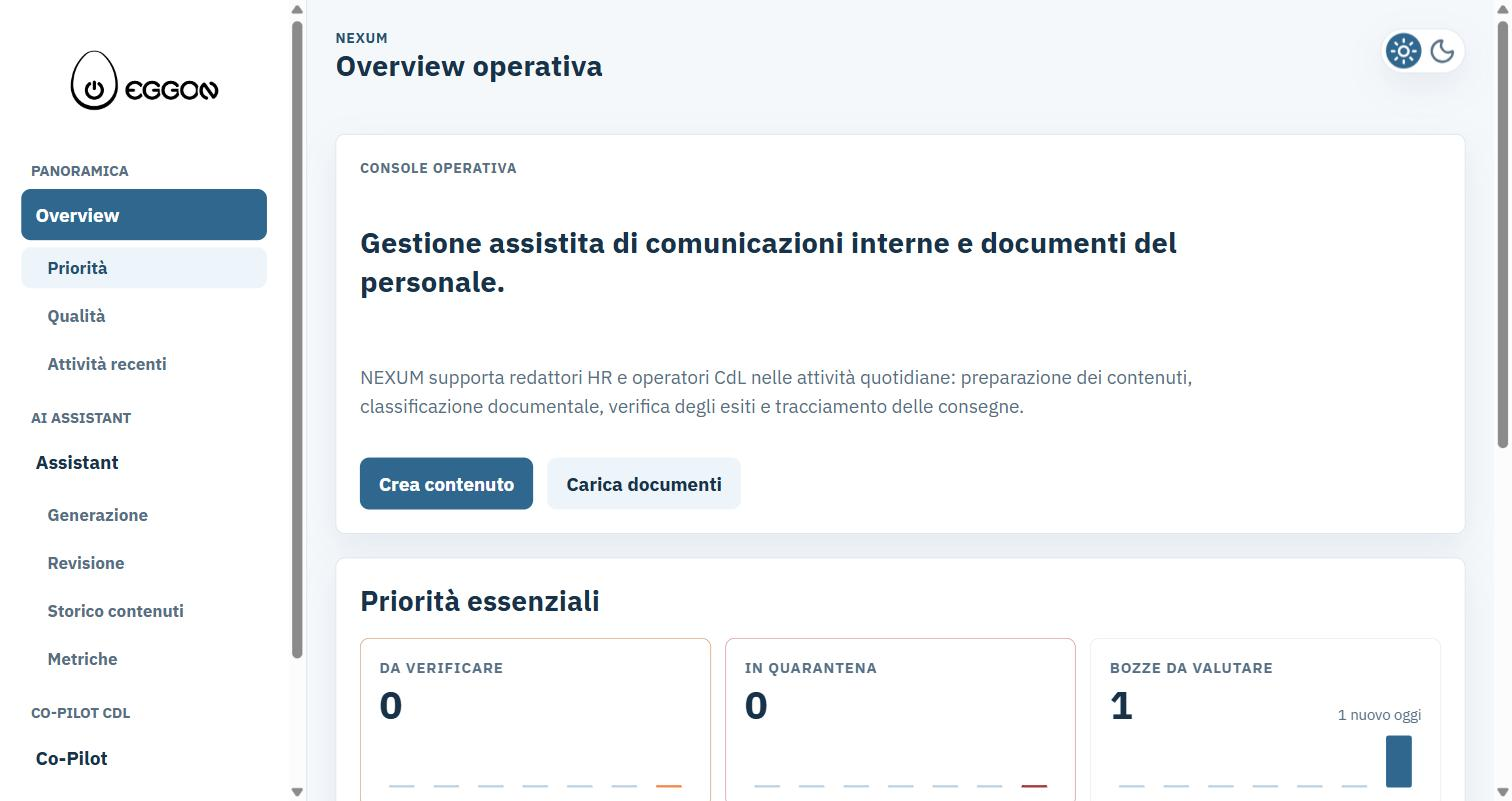
\includegraphics[width=\textwidth]{immagini/shell-completa.png}
\caption{Cornice dell'applicazione con barra laterale e intestazione}
\label{fig:shell-completa}
\end{figure}

\subsubsection{Navigazione}

\begin{itemize}
    \item \ui{Overview} apre la console di sintesi (\texttt{/overview}).
    \item \ui{Assistant} apre il modulo generativo (\texttt{/assistant}). I sotto-collegamenti portano a \ui{Generazione}, \ui{Revisione} e \ui{Storico contenuti}.
    \item \ui{Co-Pilot} apre il modulo documentale (\texttt{/copilot}). I sotto-collegamenti portano a \ui{Caricamento}, \ui{Storico documenti} e \ui{Metriche}.
\end{itemize}

I collegamenti profondi funzionano: l'indirizzo \path{https://localhost:8443/assistant} riapre direttamente l'Assistant.

\begin{figure}[H]
\centering
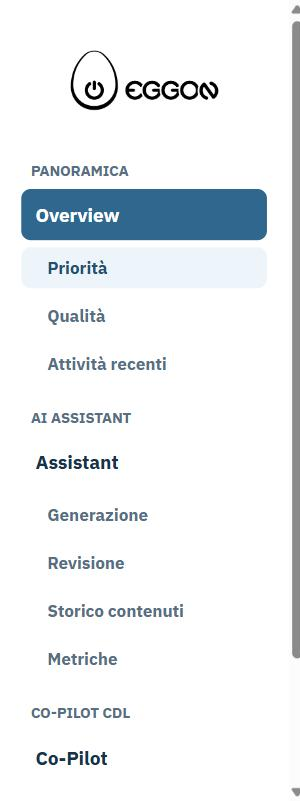
\includegraphics[width=0.4\textwidth]{immagini/sidebar-navigazione.png}
\caption{Barra laterale di navigazione}
\label{fig:sidebar-navigazione}
\end{figure}

\subsubsection{Cambio tema}

Il pulsante sole/luna nell'intestazione commuta il tema. L'etichetta accessibile è \ui{Attiva tema scuro} oppure \ui{Attiva tema chiaro}. La scelta è locale al browser.

\begin{figure}[H]
\centering

\includegraphics[width=\textwidth]{immagini/header-tema.png}
\caption{Intestazione con selettore del tema}
\label{fig:header-tema}
\end{figure}

\subsection{Overview operativa}

All'apertura si vede la console di sintesi. Non è una \glslink{dashboard}{dashboard} analitica: serve a capire lo stato corrente e a entrare nei due flussi di lavoro.

\subsubsection{Avvio rapido}

Il riquadro iniziale recita: \textit{``Gestione assistita di comunicazioni interne e documenti del personale.''} Due pulsanti scorciano i flussi:

\begin{itemize}
    \item \ui{Crea contenuto} porta alla sezione di generazione dell'Assistant.
    \item \ui{Carica documenti} porta alla sezione di caricamento del Co-Pilot.
\end{itemize}

Sotto, la sezione \ui{Da dove partire} riassume i tre punti d'ingresso: Assistant, Co-Pilot e metriche operative (queste ultime restano dentro le pagine degli strumenti, non in una vista analytics separata).

\begin{figure}[H]
\centering
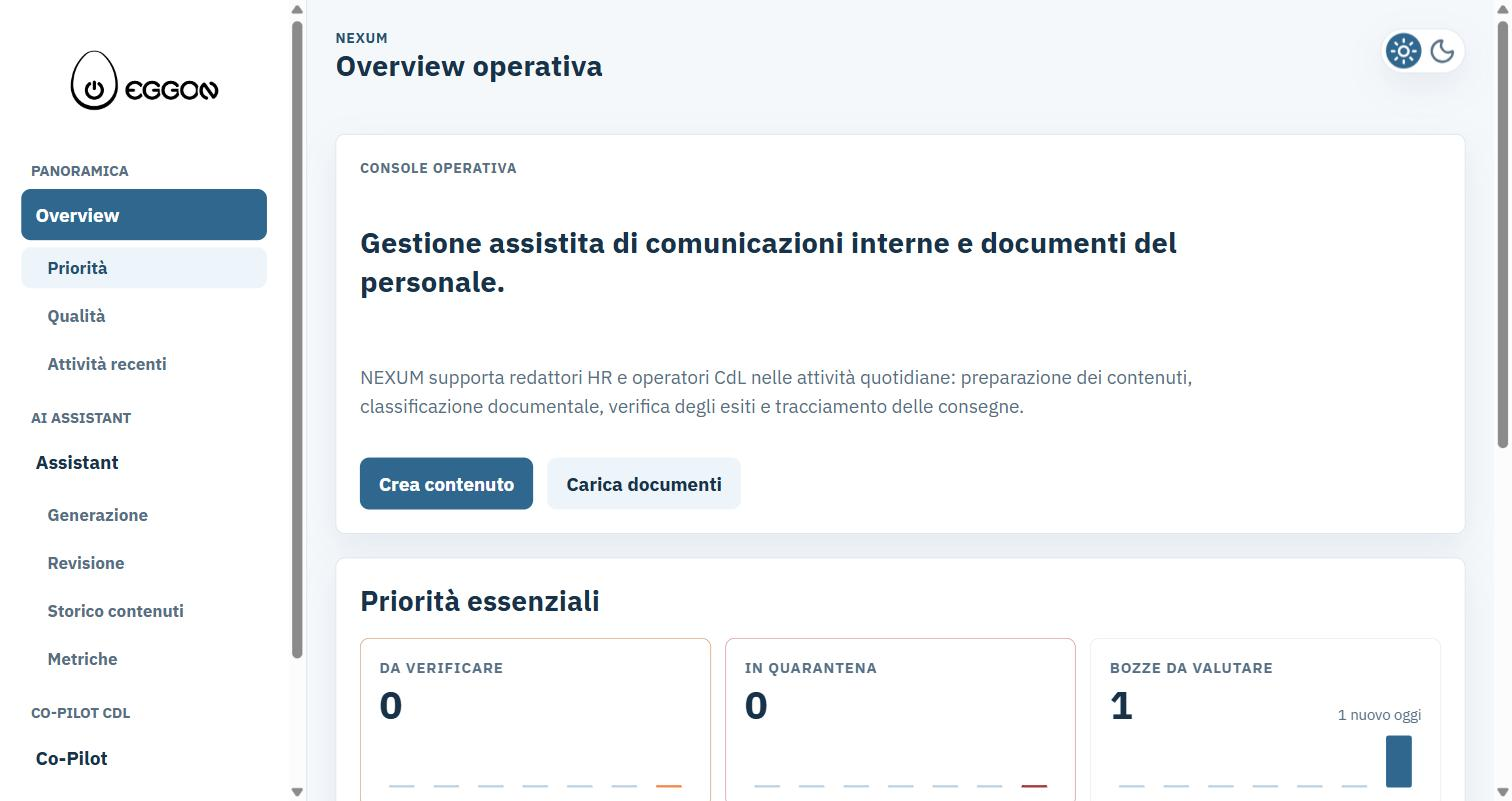
\includegraphics[width=\textwidth]{immagini/overview-hero.png}
\caption{Overview: avvio rapido}
\label{fig:overview-hero}
\end{figure}

\subsubsection{Priorità e metriche}

La sezione \ui{Priorità essenziali} mostra tre conteggi sul tenant, non sulla sola pagina visibile:

\begin{itemize}
    \item \ui{Bozze generate}: comunicazioni ancora in stato di bozza.
    \item \ui{Documenti da verificare}: sotto-documenti in attesa di revisione umana.
    \item \ui{Documenti pronti}: sotto-documenti validati automaticamente o a mano (la quarantena non conta come ``pronto'').
\end{itemize}

Più in basso, \ui{Metriche strumenti} ripete i pannelli dell'Assistant e del Co-Pilot. \ui{Attività recenti} elenca le ultime comunicazioni conservate nello storico, con titolo, stato e data di creazione. Se non c'è nulla, compare il messaggio \textit{``Le nuove attività compariranno qui.''}

Un errore di caricamento mostra un riquadro con pulsante \ui{Riprova}.

\begin{figure}[H]
\centering
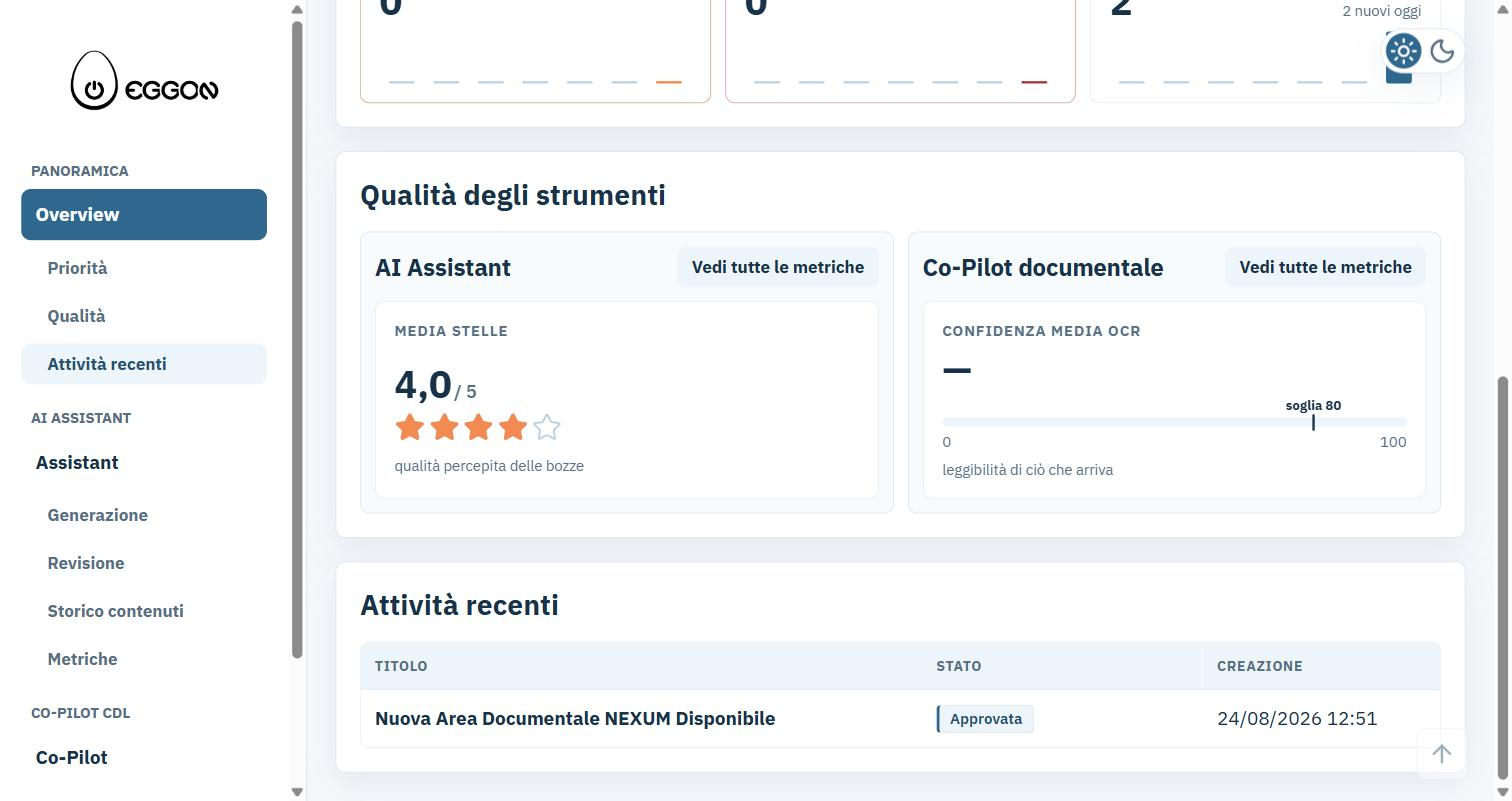
\includegraphics[width=\textwidth]{immagini/overview-metriche.png}
\caption{Overview: priorità, metriche e attività recenti}
\label{fig:overview-metriche}
\end{figure}

\subsection{AI Assistant Generativo}

Il modulo prepara comunicazioni interne a partire da un \glslink{prompt}{prompt}, da un \glslink{tono-comunicativo}{tono} e da uno \glslink{stile-editoriale}{stile}. La generazione è asincrona: l'interfaccia accetta la richiesta subito e aggiorna l'avanzamento in tempo reale. Il testo arriva per primo, la copertina dopo. Senza testo la bozza è fallita; senza copertina la bozza resta valida.

La pagina è divisa in tre blocchi, nello stesso ordine in cui si lavora: composizione, revisione, storico.

\subsubsection{Composizione della bozza}

La sezione \ui{Crea una bozza} contiene:

\begin{itemize}
    \item il campo \ui{Prompt}, obbligatorio, da 12 a 5000 caratteri. Deve descrivere cosa comunicare (destinatari interni, obiettivo, vincoli di contenuto). Un testo troppo corto impedisce l'invio;
    \item il menu \ui{Tono}, con i valori fissi \ui{Chiaro e diretto}, \ui{Più istituzionale}, \ui{Più sintetico}, \ui{Empatico}, \ui{Tecnico};
    \item il menu \ui{Stile}, con i valori fissi \ui{Testo informativo}, \ui{Avviso operativo}, \ui{Aggiornamento breve};
    \item il pulsante \ui{Genera bozza}. Durante l'elaborazione l'etichetta diventa \ui{Generazione} e il pulsante si disabilita.
\end{itemize}

Non è possibile aggiungere toni o stili personalizzati, né selezionare un'azienda di riferimento: i tre parametri sono quelli mostrati.

Sotto il form, \ui{Salva configurazione} memorizza prompt, tono e stile come preset riutilizzabile, senza avviare una generazione. Si può assegnare un nome (al massimo 150 caratteri) oppure lasciarlo vuoto: in quel caso il sistema attribuisce un'etichetta progressiva del tipo \texttt{Senza nome (1)}. Se il nome è già usato, viene comunque assegnata un'etichetta progressiva. Il pulsante è disabilitato finché il prompt non è valido.

\begin{figure}[H]
\centering
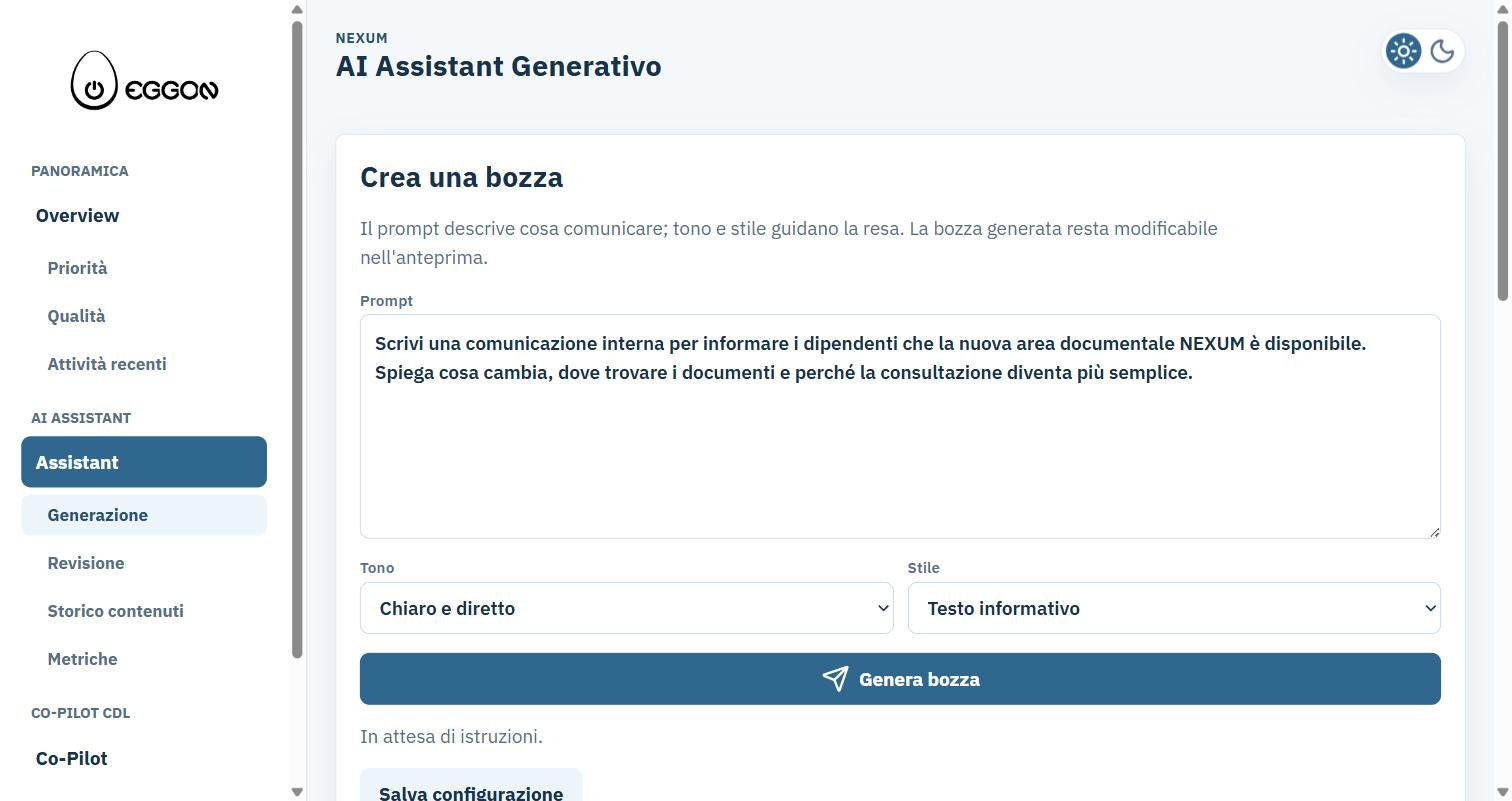
\includegraphics[width=\textwidth]{immagini/assistant-composizione.png}
\caption{Modulo di generazione della bozza}
\label{fig:assistant-composizione}
\end{figure}

\subsubsection{Avanzamento della generazione}

Dopo l'invio compare una barra di avanzamento e un messaggio di stato. Le fasi, nell'ordine, sono:

\begin{enumerate}
    \item \textit{Generazione in coda.}
    \item \textit{Generazione del testo in corso.}
    \item \textit{Testo generato. Generazione copertina in corso.}
    \item \textit{Copertina generata.} oppure \textit{Copertina non disponibile.}
    \item \textit{Bozza generata correttamente.}
\end{enumerate}

Se la richiesta resta in lavorazione a lungo, può comparire \textit{``Generazione ancora in corso. Lo stato verrà aggiornato.''} In caso di errore (modello irraggiungibile, credenziali, risposta non valida) lo stato diventa un messaggio di fallimento e la bozza non è utilizzabile. Non vengono mai mostrati testi di ripiego.

\begin{figure}[H]
\centering
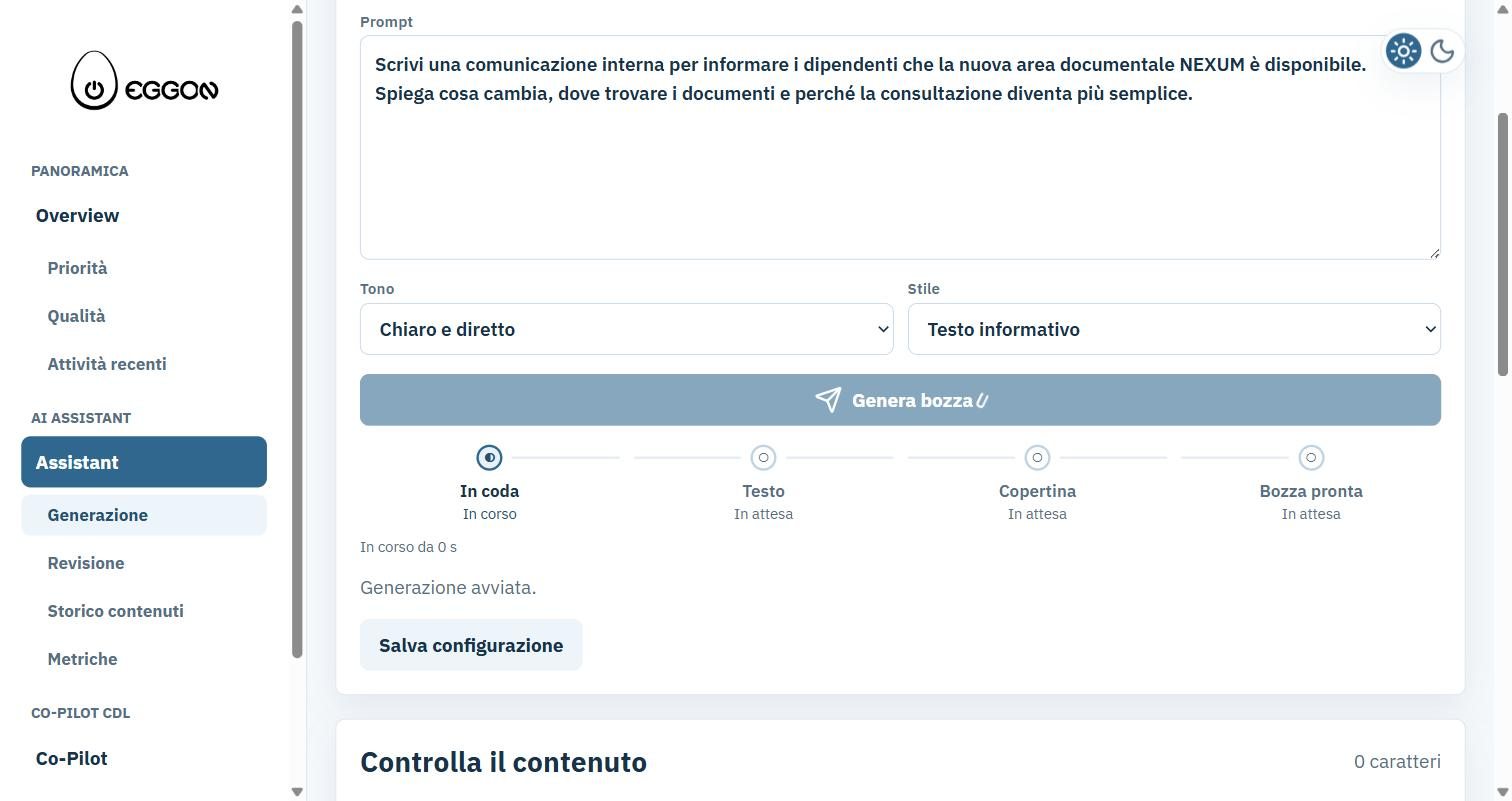
\includegraphics[width=\textwidth]{immagini/assistant-avanzamento.png}
\caption{Barra di avanzamento della generazione}
\label{fig:assistant-avanzamento}
\end{figure}

\subsubsection{Revisione del contenuto}

La sezione \ui{Controlla il contenuto} mostra la bozza corrente, oppure il record dello storico selezionato. In assenza di bozza compare \textit{``La bozza generata apparira qui.''}

Quando la bozza è pronta si vedono, dall'alto:

\begin{itemize}
    \item l'immagine di copertina, se presente. Durante la generazione compare \textit{``Generazione copertina in corso.''}; se manca o è stata tolta, \textit{``Nessuna copertina per questa bozza.''}; se la generazione dell'immagine è fallita, un avviso con il motivo;
    \item i pulsanti \ui{Cambia immagine} e \ui{Rimuovi immagine} (assenti se la bozza è stata scartata). L'immagine sostitutiva deve essere PNG, JPEG o WebP, massimo 5~MB;
    \item i campi \ui{Titolo} (massimo 255 caratteri) e \ui{Testo} (massimo 20\,000 caratteri), in sola lettura finché non si preme \ui{Modifica};
    \item il blocco \ui{Documento finale}, visibile solo a generazione conclusa e se la bozza non è scartata: \ui{Apri anteprima} (nuova scheda) e \ui{Scarica PDF}. Ogni pagina del documento riporta il \glslink{marcatore-di-trasparenza}{marcatore di trasparenza} \textit{``Creato da AI Assistant''};
    \item la valutazione a stelle (paragrafo successivo);
    \item lo stato della bozza (\ui{Bozza}, \ui{Approvata} o \ui{Scartata}) e la dicitura \textit{``Creato da AI Assistant''};
    \item le azioni \ui{Salva nello storico}, \ui{Rigenera bozza} e \ui{Scarta bozza}.
\end{itemize}

\begin{figure}[H]
\centering
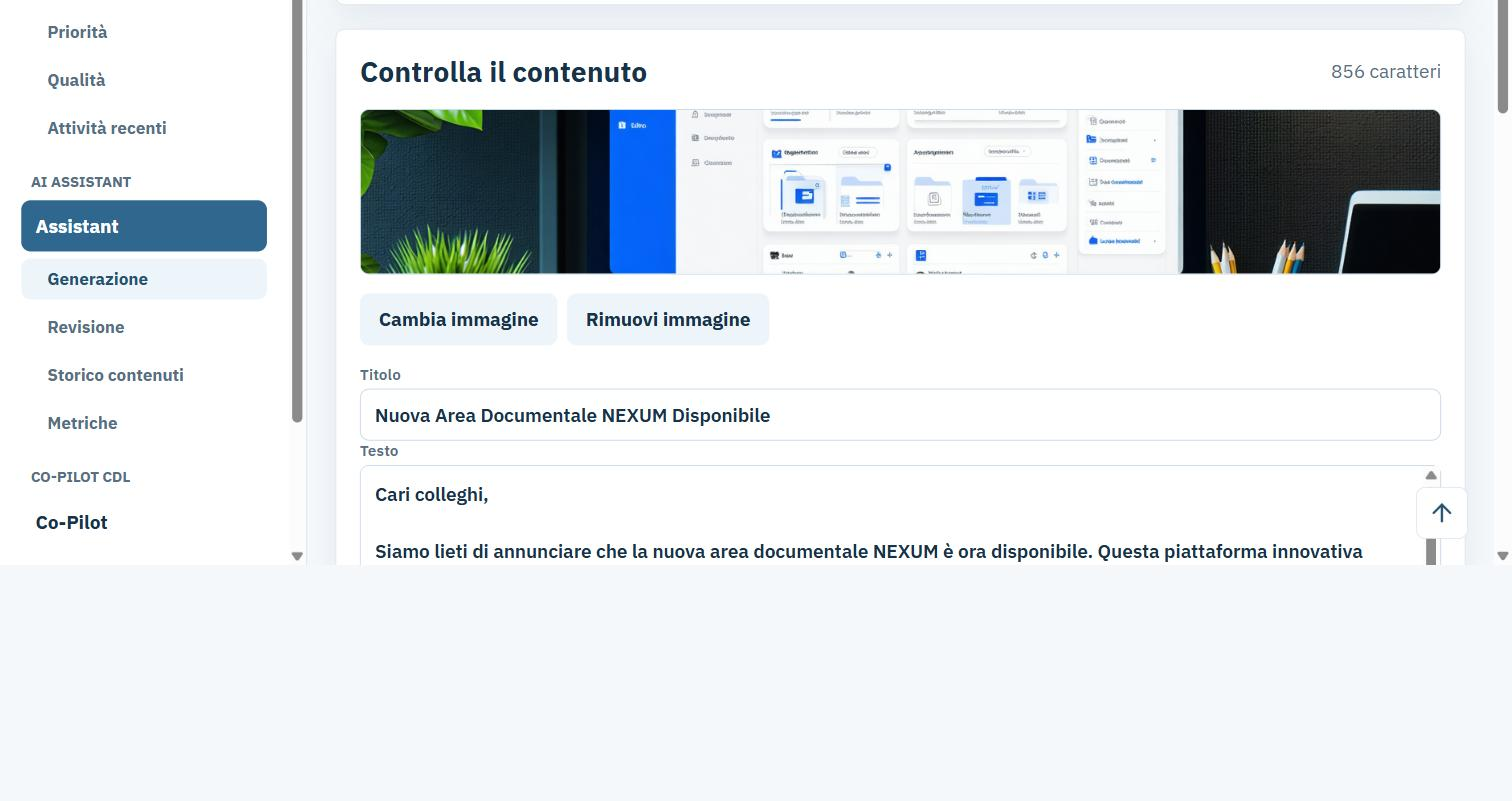
\includegraphics[width=\textwidth]{immagini/assistant-revisione.png}
\caption{Anteprima della bozza generata}
\label{fig:assistant-revisione}
\end{figure}

\paragraph{Modifica di titolo e testo}

\ui{Modifica} abilita i due campi. \ui{Salva} persiste le correzioni; \ui{Annulla} le scarta e ripristina i valori precedenti. La modifica è consentita finché la bozza non è \ui{Scartata}, anche dopo il salvataggio nello storico. Una rigenerazione sostituisce titolo, testo e copertina e chiude un'eventuale modifica non salvata.

\begin{figure}[H]
\centering
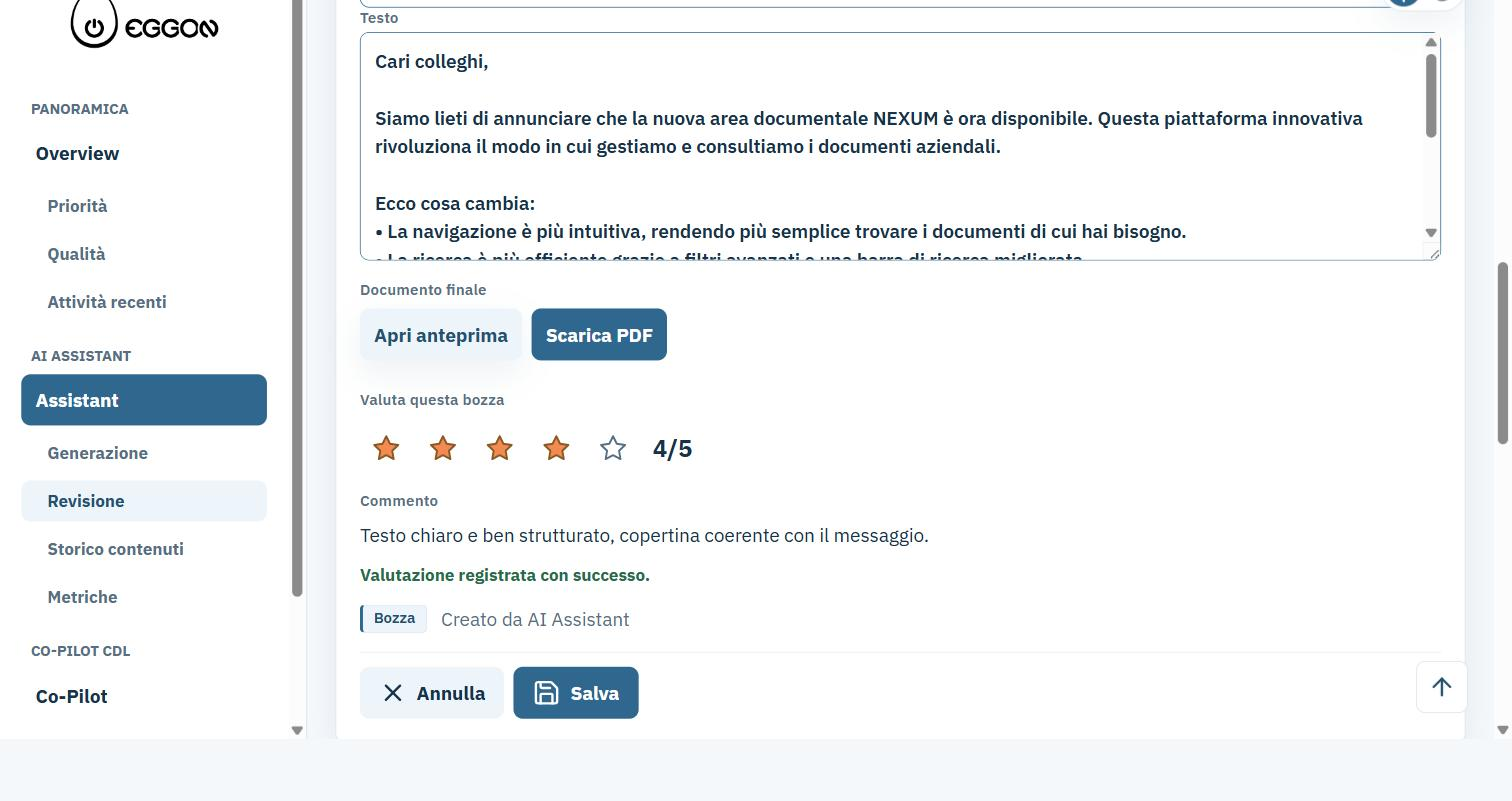
\includegraphics[width=\textwidth]{immagini/assistant-modifica.png}
\caption{Bozza in modalità modifica}
\label{fig:assistant-modifica}
\end{figure}

\paragraph{Valutazione}

Ogni generazione si valuta una sola volta, da 1 a 5 stelle, con un commento facoltativo di al massimo 1000 caratteri. Si selezionano le stelle, si scrive eventualmente il commento e si conferma con \ui{Invia valutazione}. Senza un punteggio il pulsante resta disabilitato. Dopo l'invio compare \textit{``Valutazione registrata con successo.''} e, se presente, il commento salvato. La valutazione non è modificabile e non è obbligatoria per salvare nello storico.

\begin{figure}[H]
\centering
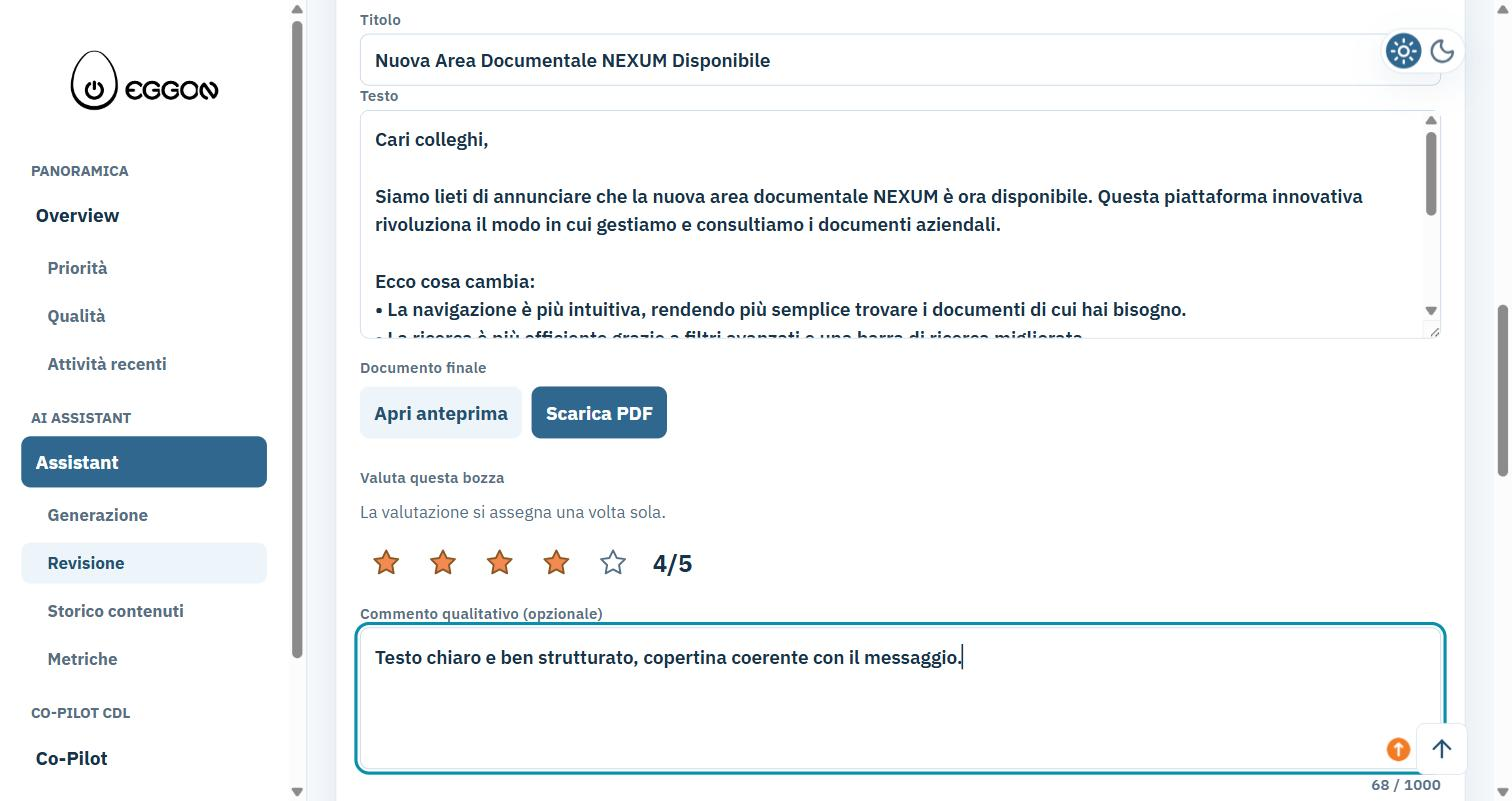
\includegraphics[width=\textwidth]{immagini/assistant-valutazione.png}
\caption{Valutazione a stelle della bozza}
\label{fig:assistant-valutazione}
\end{figure}

\paragraph{Salvataggio nello storico, rigenerazione e scarto}

\begin{itemize}
    \item \ui{Salva nello storico} sposta la bozza nello stato \ui{Approvata} e la fa comparire nello storico. Finché non si preme, la generazione resta nell'area di lavoro e non compare nell'elenco. Il salvataggio non congela il contenuto: titolo, testo e copertina restano modificabili e la bozza resta rigenerabile. Il pulsante scompare quando lo stato è già \ui{Approvata}.
    \item \ui{Rigenera bozza} chiede una nuova variante con gli stessi prompt, tono e stile. Sostituisce testo e copertina della bozza corrente. È disponibile anche dopo il salvataggio nello storico, non su una bozza scartata.
    \item \ui{Scarta bozza} chiede conferma: \textit{``Sei sicuro di voler scartare questa bozza? Non sarà più modificabile né rigenerabile.''} Con \ui{Conferma eliminazione} lo stato diventa \ui{Scartata}: la bozza resta tracciata ma esce dallo storico attivo. \ui{Annulla} chiude la richiesta di conferma.
\end{itemize}

\begin{figure}[H]
\centering
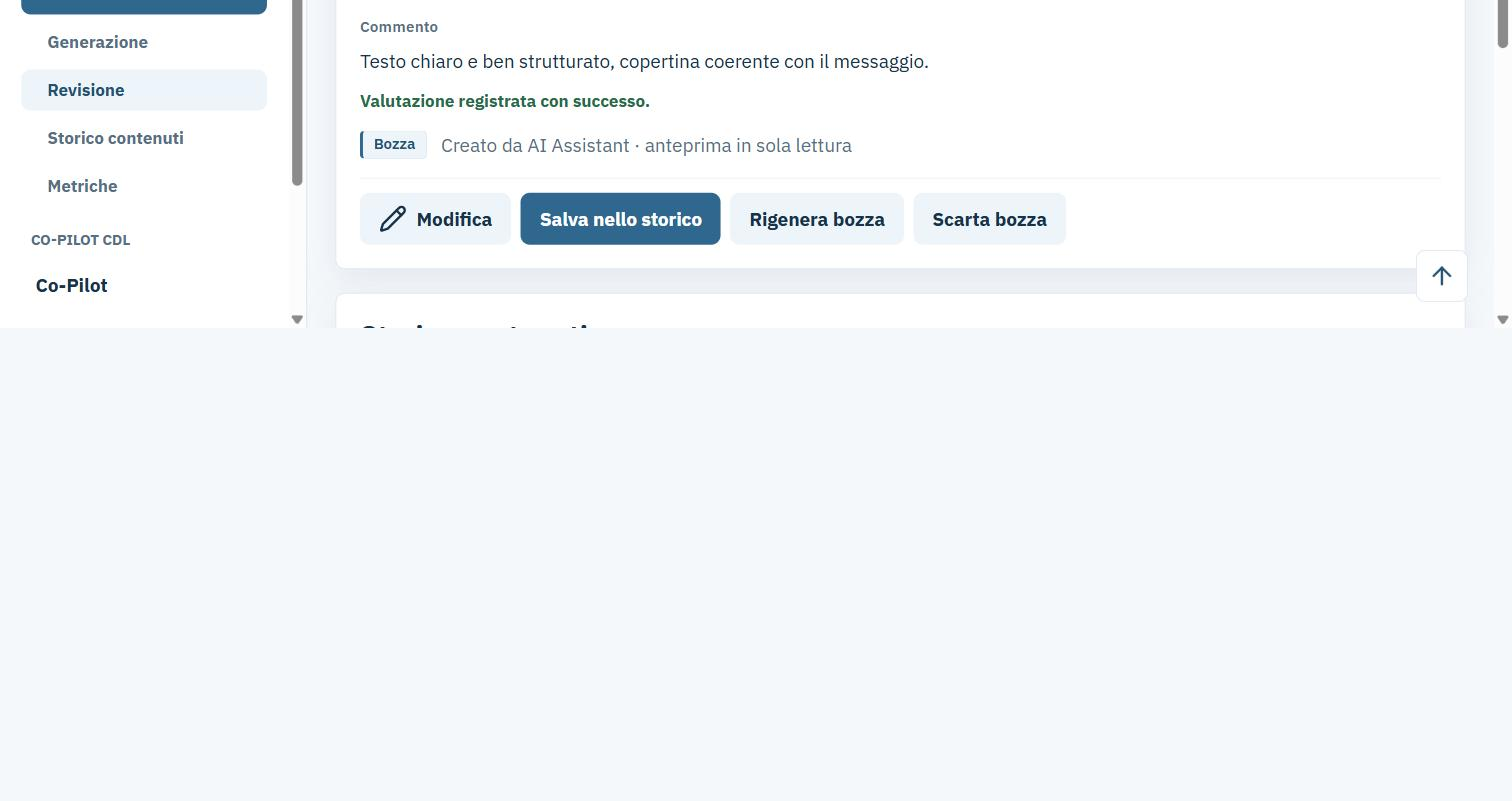
\includegraphics[width=\textwidth]{immagini/assistant-azioni.png}
\caption{Azioni sulla bozza: storico, rigenerazione, scarto}
\label{fig:assistant-azioni}
\end{figure}

\subsubsection{Storico contenuti}

La sezione \ui{Storico contenuti} elenca solo le comunicazioni in stato \ui{Approvata}. Una bozza appena generata, o una bozza scartata, non vi compare. Accanto al titolo della sezione è indicato il numero di record.

\paragraph{Filtri}

I filtri si applicano sia alle comunicazioni sia alle configurazioni salvate, con un breve ritardo di digitazione:

\begin{itemize}
    \item \ui{Parola chiave}: cerca nel prompt (e, per i preset, anche nel nome);
    \item \ui{Tono} e \ui{Stile}: gli stessi elenchi del form di generazione, più l'opzione ``tutti'';
    \item \ui{Data}: giorno di creazione;
    \item \ui{Azzera filtri} ripulisce tutti i campi.
\end{itemize}

Se i filtri non trovano nulla, compare \textit{``Nessuna comunicazione corrisponde ai filtri selezionati.''} Senza filtri e senza record: \textit{``Le bozze generate compariranno qui.''}

\begin{figure}[H]
\centering

\includegraphics[width=\textwidth]{immagini/assistant-filtri.png}
\caption{Filtri dello storico contenuti}
\label{fig:assistant-filtri}
\end{figure}

\paragraph{Configurazioni salvate}

Sopra le card delle comunicazioni, se esistono preset che superano i filtri, compare il blocco \ui{Configurazioni salvate}. Ogni riga mostra nome, data, \ui{Usa} e l'icona di eliminazione.

\begin{itemize}
    \item \ui{Usa} ricompila il form di generazione con prompt, tono e stile del preset. Non avvia una nuova generazione. Non si applica a una bozza già salvata nello storico: su quella restano modifica e rigenerazione dirette.
    \item L'icona cestino chiede \textit{``Eliminare definitivamente questa configurazione salvata?''} con \ui{Conferma eliminazione} e \ui{Annulla}.
\end{itemize}

\begin{figure}[H]
\centering
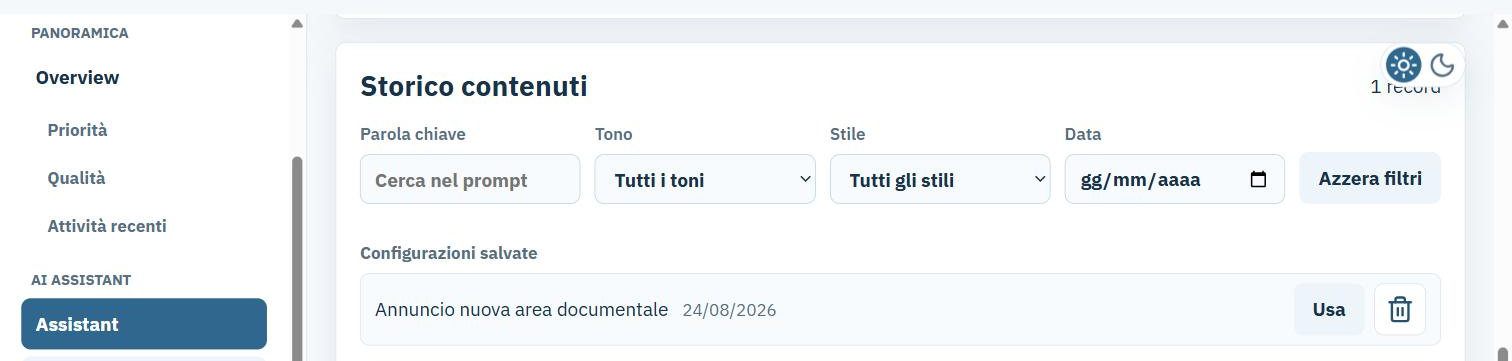
\includegraphics[width=\textwidth]{immagini/assistant-configurazioni.png}
\caption{Preset di prompt salvati}
\label{fig:assistant-configurazioni}
\end{figure}

\paragraph{Card dello storico}

Ogni comunicazione è una card con badge di stato, titolo e data. Un clic sulla card la seleziona e la carica nell'anteprima di revisione (la card selezionata resta evidenziata).

In basso a destra:

\begin{itemize}
    \item l'icona a stella aggiunge o toglie la voce dai preferiti (\glslink{bookmark}{bookmark}). L'etichetta accessibile è \ui{Aggiungi ai preferiti} o \ui{Rimuovi dai preferiti};
    \item l'icona cestino chiede \textit{``Eliminare definitivamente questo elemento dallo storico?''}. La conferma rimuove il record in modo irreversibile.
\end{itemize}

\begin{figure}[H]
\centering
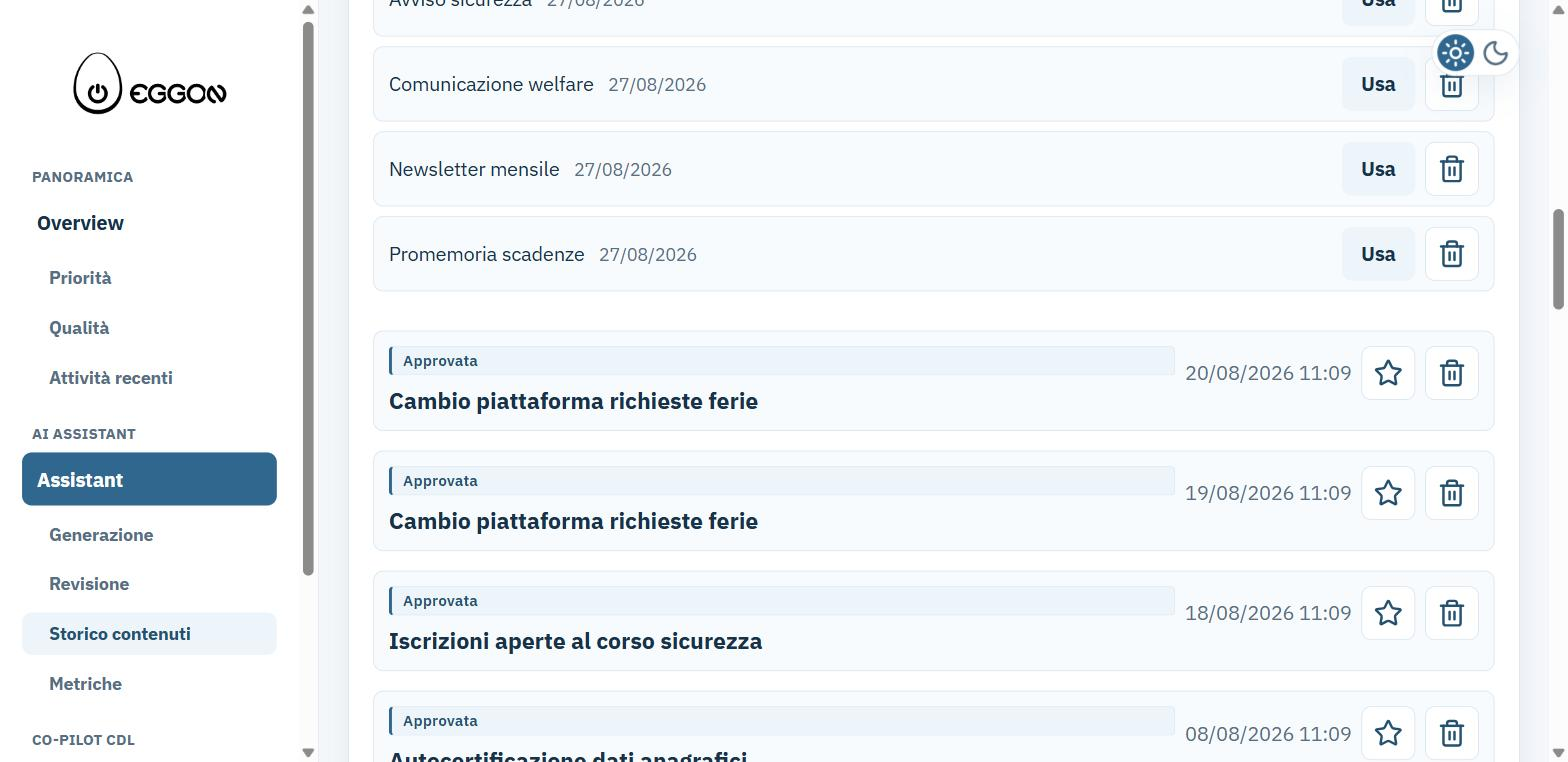
\includegraphics[width=\textwidth]{immagini/assistant-storico.png}
\caption{Elenco dello storico contenuti}
\label{fig:assistant-storico}
\end{figure}

\subsubsection{Stati della comunicazione}

\begin{center}
\renewcommand{\arraystretch}{1.25}
\begin{tabularx}{\textwidth}{|p{3.2cm}|X|}
\hline
\rowcolor{gray!20}
\textbf{Stato} & \textbf{Significato per l'utente} \\
\hline
\ui{Bozza} & Generazione conclusa (o in corso) nell'area di lavoro. Non compare nello storico. \\
\hline
\ui{Approvata} & Il redattore l'ha salvata nello storico. Resta modificabile e rigenerabile. Non è una validazione da parte di un altro ruolo. \\
\hline
\ui{Scartata} & Esclusa dallo storico attivo. Non più modificabile né rigenerabile. \\
\hline
\end{tabularx}
\end{center}

\subsection{AI Co-Pilot per i Consulenti del Lavoro}

Il modulo analizza un PDF di qualsiasi tipologia, riconosce almeno un destinatario, eventuale \glslink{split-automatico}{split} in sotto-documenti e estrae i campi principali. Dopo l'analisi l'operatore interviene in ottica \glslink{human-in-the-loop}{human-in-the-loop}: corregge, valida e prepara il messaggio di invio. L'invio vero e proprio resta fuori dalla piattaforma.

\subsubsection{Caricamento}

La sezione \ui{Carica nel repository} accetta un solo file per volta. Prima del file si possono indicare dei \glslink{metadati}{metadati} facoltativi. Quello che viene dichiarato qui \textbf{fa fede}: l'AI continua a produrre la propria estrazione, consultabile, ma tipologia, mese, anno e azienda indicati a mano non vengono sovrascritti.

\begin{itemize}
    \item \ui{Tipologia documento}: \ui{cedolino}, \ui{CU}, \ui{comunicazione}, \ui{documento da firmare}, \ui{lettera}, \ui{altro}. Un secondo clic sulla stessa tipologia la deseleziona.
    \item \ui{Mese di riferimento}: elenco dei mesi, oppure \ui{Automatico (AI)}.
    \item \ui{Anno di riferimento}: numero compreso fra 1900 e 2100.
    \item \ui{Azienda}: testo libero, massimo 500 caratteri.
\end{itemize}

L'area tratteggiata \ui{Seleziona o trascina un documento} apre il selettore file. È accettato solo \texttt{application/pdf}. Durante l'upload i metadati si disabilitano.

Vincoli sul file, oltre al formato:

\begin{itemize}
    \item dimensione massima 20~MB (valore di default);
    \item massimo 50 pagine;
    \item PDF non cifrato e non protetto da password;
    \item firma PDF valida e file strutturalmente leggibile;
    \item nome file senza percorsi o caratteri non consentiti.
\end{itemize}

Un rifiuto viene mostrato come errore applicativo (ad esempio \textit{``I PDF cifrati o protetti da password non sono supportati.''}).

\begin{figure}[H]
\centering
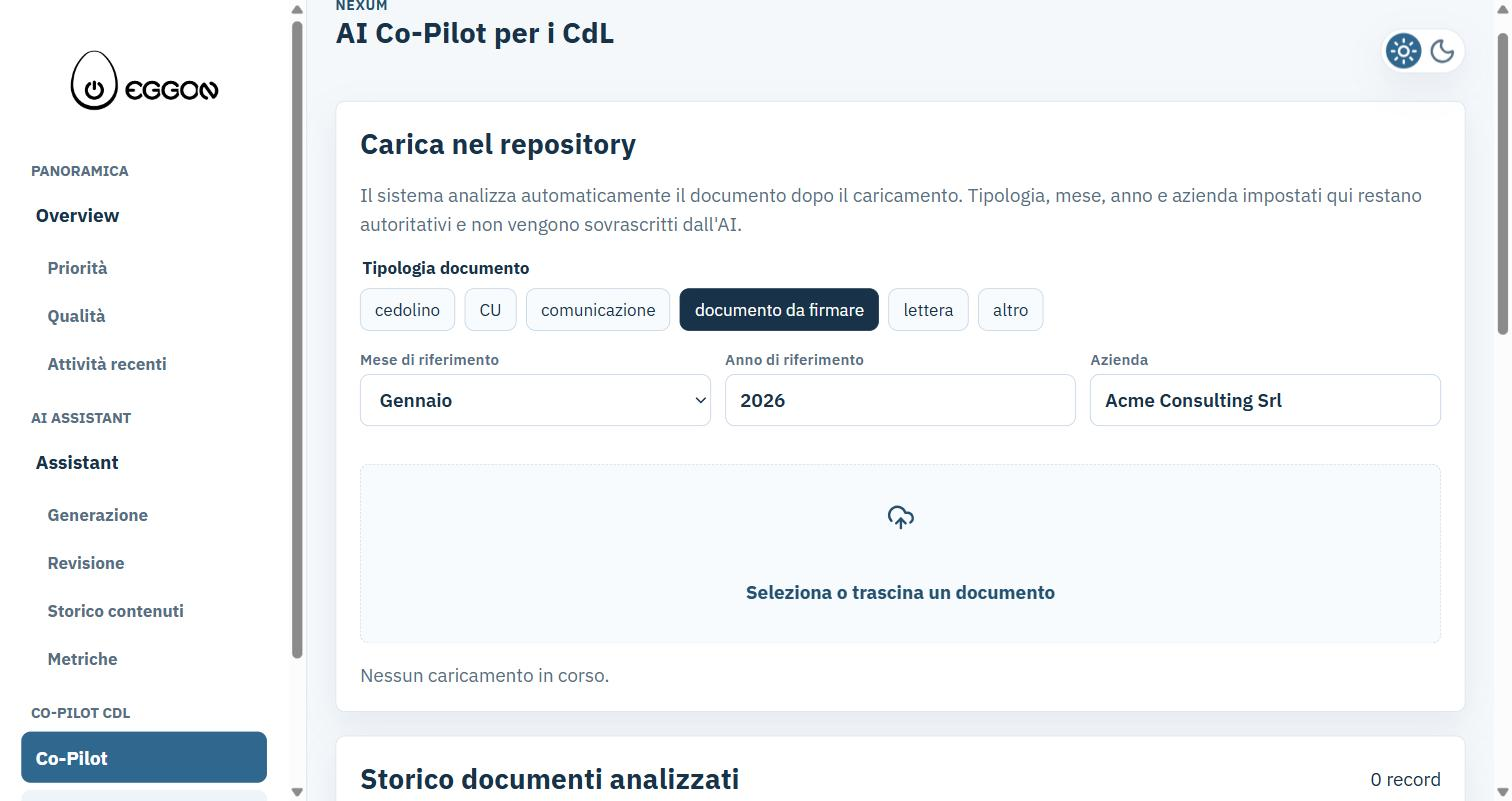
\includegraphics[width=\textwidth]{immagini/copilot-caricamento.png}
\caption{Pannello di caricamento documenti}
\label{fig:copilot-caricamento}
\end{figure}

\subsubsection{Avanzamento dell'elaborazione}

Dopo l'accettazione del file, una barra segue le fasi:

\begin{enumerate}
    \item upload in corso;
    \item \textit{Documento in coda di elaborazione;}
    \item \textit{Analisi OCR del documento in corso;}
    \item \textit{Estrazione dati dai sotto-documenti in corso;}
    \item \textit{Elaborazione completata.}
\end{enumerate}

Se l'elaborazione si prolunga può comparire \textit{``Elaborazione ancora in corso. Lo stato verrà aggiornato.''} Un fallimento di split o estrazione lascia il documento in stato \ui{Fallito}, con un messaggio nell'area di dettaglio. Non vengono inventati destinatari o campi per mascherare l'errore.

\begin{figure}[H]
\centering
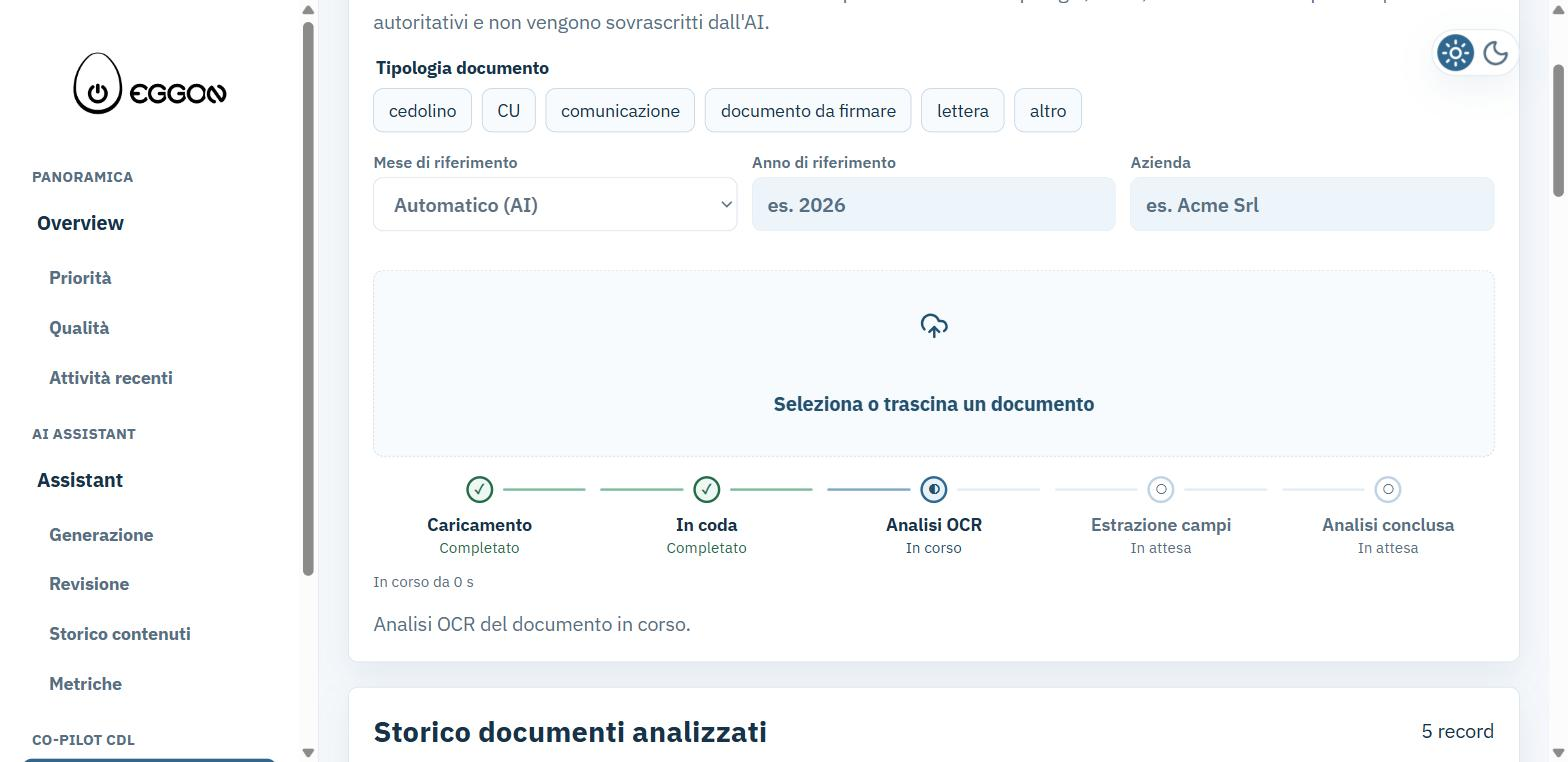
\includegraphics[width=\textwidth]{immagini/copilot-avanzamento.png}
\caption{Avanzamento dell'analisi documentale}
\label{fig:copilot-avanzamento}
\end{figure}

\subsubsection{Storico documenti analizzati}

La sezione \ui{Storico documenti analizzati} elenca i sotto-documenti del tenant. Ogni riga mostra:

\begin{itemize}
    \item destinatario (nome e cognome) e azienda;
    \item titolo o tipologia;
    \item nome file;
    \item data del documento;
    \item data e ora di caricamento;
    \item \glslink{confidenza-confidence-score}{confidenza} in percentuale, oppure \ui{Da verificare} se non ancora calcolata;
    \item stato di revisione;
    \item stato di invio;
    \item pulsante \ui{Consulta}, che apre il dettaglio sotto la tabella (il pulsante della riga selezionata resta evidenziato).
\end{itemize}

Senza documenti: \textit{``I documenti caricati compariranno qui.''}

\begin{figure}[H]
\centering
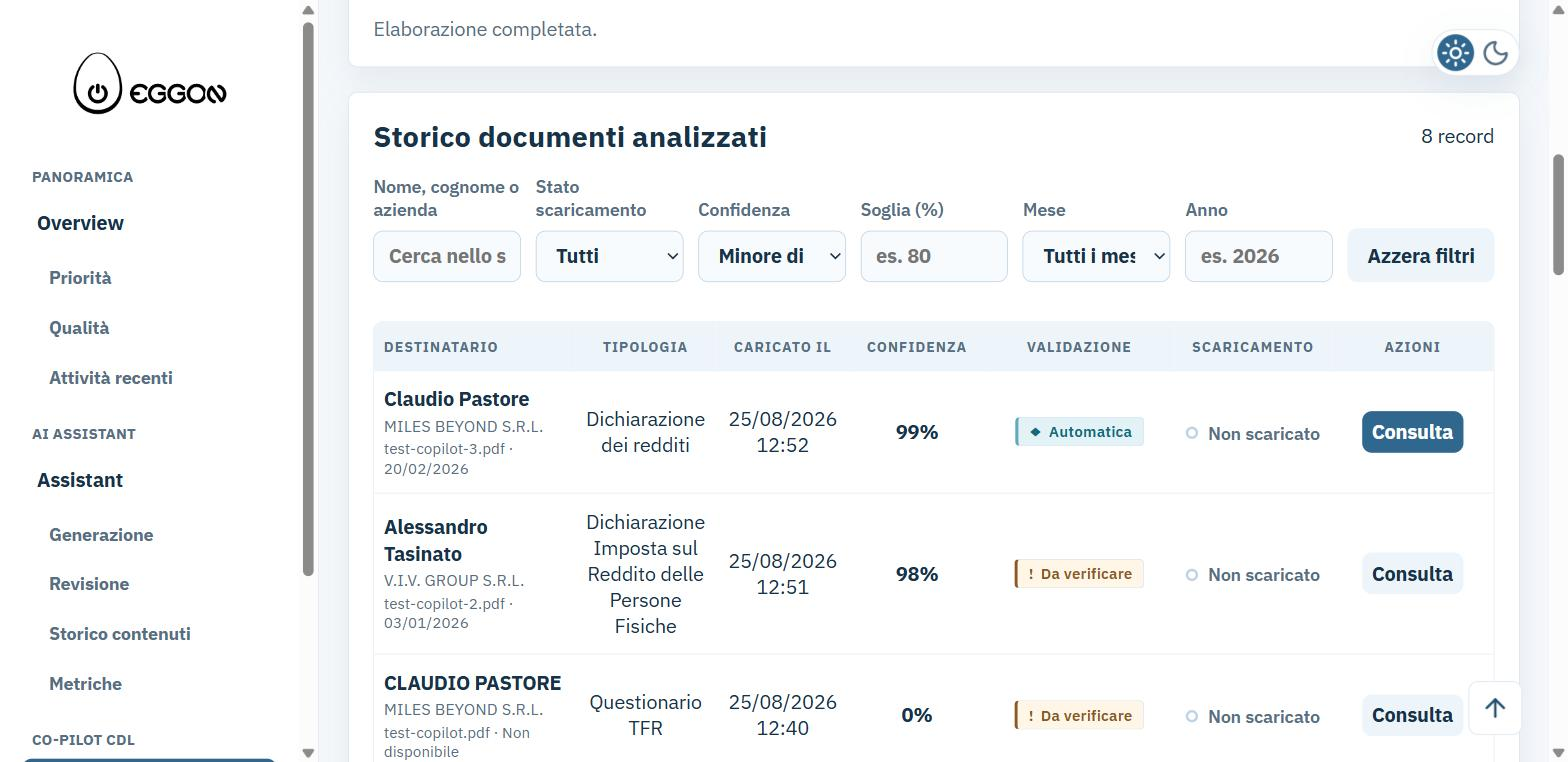
\includegraphics[width=\textwidth]{immagini/copilot-storico.png}
\caption{Tabella dello storico documenti}
\label{fig:copilot-storico}
\end{figure}

\paragraph{Filtri}

I criteri sono applicati dal backend, sul solo tenant corrente:

\begin{itemize}
    \item \ui{Nome, cognome o azienda}: ricerca testuale;
    \item \ui{Stato invio}: \ui{Inviato} o \ui{Non inviato} (in interfaccia le etichette degli stati in tabella sono \ui{Inviato} e \ui{Da inviare});
    \item \ui{Confidenza}: \ui{Minore di} o \ui{Maggiore di} una \ui{Soglia (\%)} da 0 a 100;
    \item \ui{Mese} e \ui{Anno} del documento;
    \item \ui{Azzera filtri}.
\end{itemize}

Con filtri attivi e nessun risultato: \textit{``Nessun documento corrisponde ai filtri selezionati.''}

\begin{figure}[H]
\centering
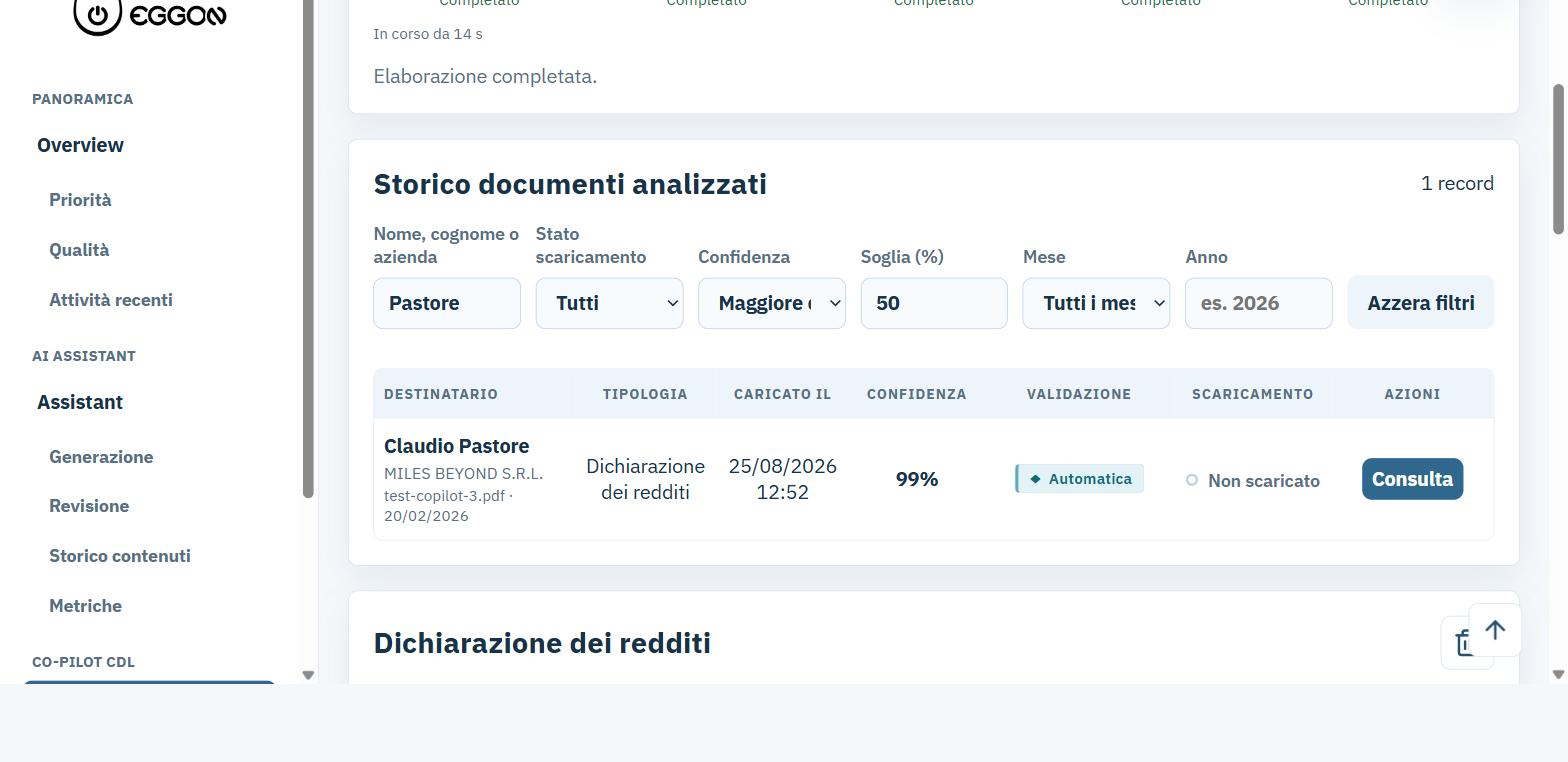
\includegraphics[width=\textwidth]{immagini/copilot-filtri.png}
\caption{Filtri dello storico documenti}
\label{fig:copilot-filtri}
\end{figure}

\subsubsection{Dettaglio e revisione}

Selezionando \ui{Consulta} si apre la sezione di verifica, con titolo del documento e, in alto a destra, l'icona cestino per eliminare il sotto-documento. Sotto, un indicatore mostra lo stato di revisione corrente.

Il dettaglio è affiancato:

\begin{itemize}
    \item \textbf{a sinistra, \ui{Anteprima documento}:} il PDF del sotto-documento in un riquadro, con collegamento \ui{Apri in una nuova scheda}. Se lo storage non è raggiungibile compare \textit{``Storage documento non raggiungibile.''}; se il file manca, \textit{``Anteprima non disponibile.''}; in attesa, \textit{``Caricamento anteprima in corso.''}
    \item \textbf{a destra, \ui{Dati estratti dall'OCR}:} i campi strutturati, con una legenda \ui{Modificabile} / \ui{Sola lettura}.
\end{itemize}

Se la confidenza è sotto l'80\% il pannello dei dati è evidenziato come da controllare con priorità.

\begin{figure}[H]
\centering

\includegraphics[width=\textwidth]{immagini/copilot-dettaglio.png}
\caption{Dettaglio documento: anteprima e dati estratti}
\label{fig:copilot-dettaglio}
\end{figure}

\paragraph{Campi in sola lettura}

\begin{itemize}
    \item nome file;
    \item numero pagine;
    \item confidenza;
    \item stato revisione;
    \item email destinatario rilevata in sola lettura (con pulsante di copia negli appunti, se valorizzata). Questa email \textbf{non} è compilata dalla pipeline OCR/Bedrock: va inserita a mano nel campo modificabile omonimo;
    \item data e ora di caricamento.
\end{itemize}

\paragraph{Campi modificabili}

\begin{itemize}
    \item nome e cognome;
    \item azienda;
    \item data documento;
    \item tipologia (l'elenco comprende le sei tipologie predefinite; se l'AI ha proposto un valore fuori elenco, quel valore resta selezionabile);
    \item descrizione;
    \item email destinatario, con controllo di formato;
    \item codice fiscale, con controllo del carattere di controllo italiano (16 caratteri; un valore formalmente invalido viene rifiutato);
    \item matricola dipendente.
\end{itemize}

Email, codice fiscale e matricola \textbf{non} sono estratti automaticamente: restano a carico dell'operatore. È coerente con l'obiettivo della \glslink{mvp-minimum-viable-product}{MVP}, che privilegia l'identificazione del destinatario (nome, contesto documentale) rispetto al recapito.

\paragraph{Come si calcola la confidenza}

La \glslink{confidenza-confidence-score}{confidenza} non è un'auto-valutazione del modello. Misura la leggibilità \glslink{ocr-riconoscimento-ottico-dei-caratteri}{OCR} ponderata sulla completezza dei campi lasciati all'AI. I metadati dichiarati in caricamento restano fuori dal calcolo: dichiarare tipologia o azienda non ``gonfia'' il punteggio. La \glslink{soglia-di-confidenza}{soglia} operativa di default è 80\%.

\paragraph{Azioni di revisione}

Fuori dalla modalità modifica:

\begin{itemize}
    \item \ui{Modifica} abilita i campi editabili;
    \item \ui{Conferma dati correnti} marca il sotto-documento come \ui{Validato manualmente} senza cambiare i valori;
    \item \ui{Invia} apre il pannello del messaggio di invio (non recapita nulla).
\end{itemize}

In modifica, \ui{Salva} persiste le correzioni e \ui{Annulla} le scarta. Gli errori di validazione compaiono sotto il campo interessato (ad esempio \textit{``Formato e-mail non valido.''} o \textit{``Il codice fiscale non supera il controllo di validità formale.''}).

\begin{figure}[H]
\centering
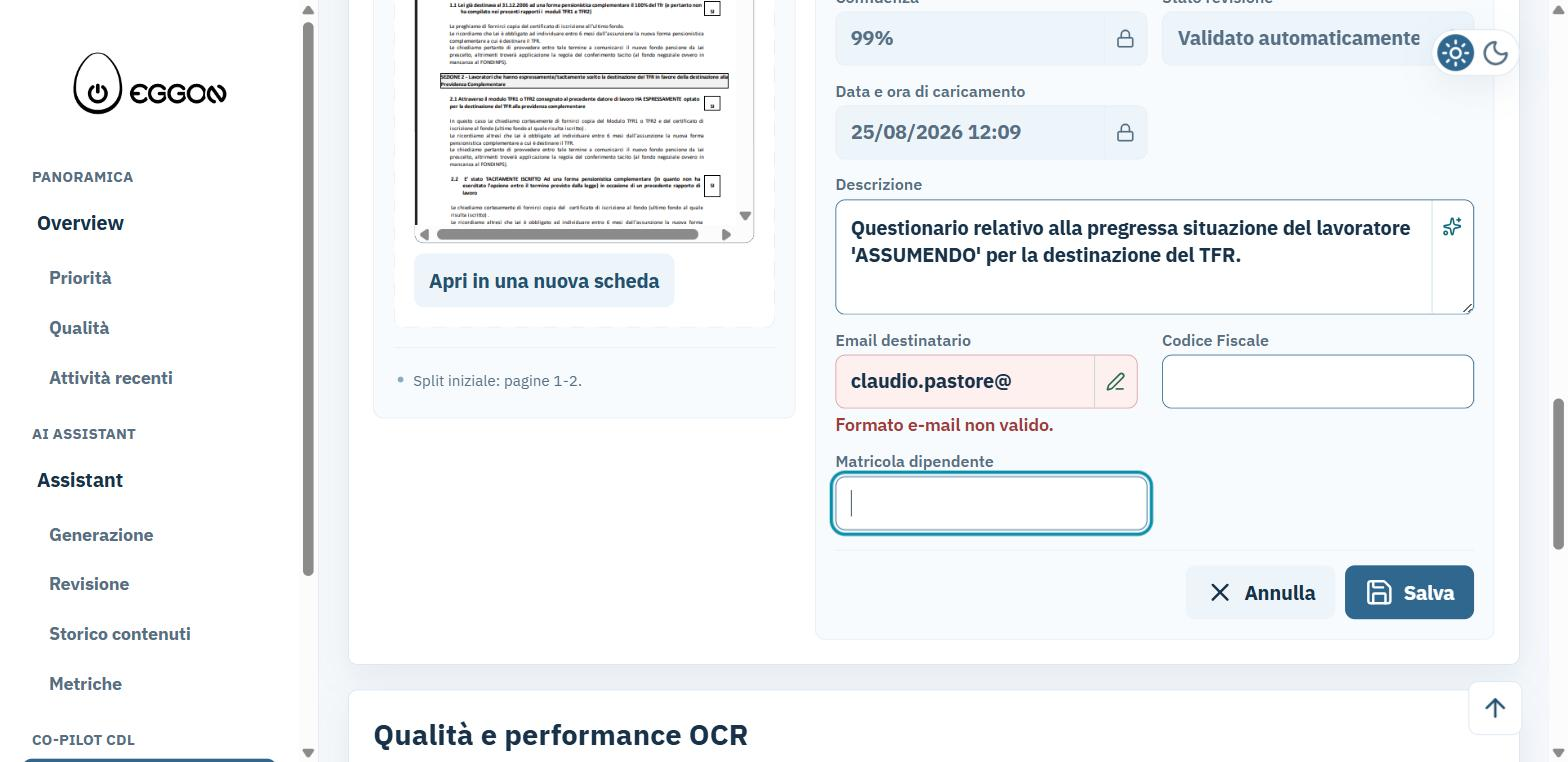
\includegraphics[width=\textwidth]{immagini/copilot-revisione.png}
\caption{Modifica dei dati estratti}
\label{fig:copilot-revisione}
\end{figure}

\subsubsection{Stati di revisione e di invio}

\begin{center}
\renewcommand{\arraystretch}{1.25}
\begin{tabularx}{\textwidth}{|p{4.8cm}|X|}
\hline
\rowcolor{gray!20}
\textbf{Stato di revisione} & \textbf{Significato} \\
\hline
\ui{Da revisionare} & L'estrazione automatica richiede un controllo umano. \\
\hline
\ui{Validato automaticamente} & I campi automatici superano la soglia di confidenza. \\
\hline
\ui{Validato manualmente} & L'operatore ha confermato o corretto i dati. \\
\hline
\ui{In quarantena} & Il sotto-documento non è utilizzabile nello stato attuale. \\
\hline
\end{tabularx}
\end{center}

\vspace{0.6em}

\begin{center}
\renewcommand{\arraystretch}{1.25}
\begin{tabularx}{\textwidth}{|p{4.4cm}|X|}
\hline
\rowcolor{gray!20}
\textbf{Stato di invio} & \textbf{Significato} \\
\hline
\ui{Da inviare} & Il PDF del messaggio non è ancora stato scaricato. \\
\hline
\ui{Inviato} & Il PDF del messaggio è stato scaricato almeno una volta. Non implica un recapito. \\
\hline
\end{tabularx}
\end{center}

Lo stato di elaborazione del documento originale (\ui{In attesa}, \ui{In elaborazione}, \ui{Completato}, \ui{Fallito}) riguarda la pipeline, non la revisione del singolo sotto-documento.

\subsubsection{Messaggio di invio}

Il pulsante \ui{Invia} apre il blocco \ui{Messaggio di invio}, precompilato da destinatario, oggetto e testo calcolati sui dati estratti. I tre campi sono modificabili. \ui{Salva} persiste le correzioni; \ui{Annulla} ripristina i valori precedenti; la X chiude il pannello.

Sotto i campi, in sola lettura:

\begin{itemize}
    \item \ui{Apri anteprima} mostra il PDF impaginato del messaggio;
    \item \ui{Scarica PDF} scarica quel PDF. Il primo scaricamento fa passare lo stato di invio a \ui{Inviato}. Uno scaricamento successivo non lo riporta indietro.
\end{itemize}

Il recapito al dipendente avviene fuori da NEXUM (posta elettronica dello studio, altri canali). La piattaforma si ferma alla preparazione del plico.

\begin{figure}[H]
\centering
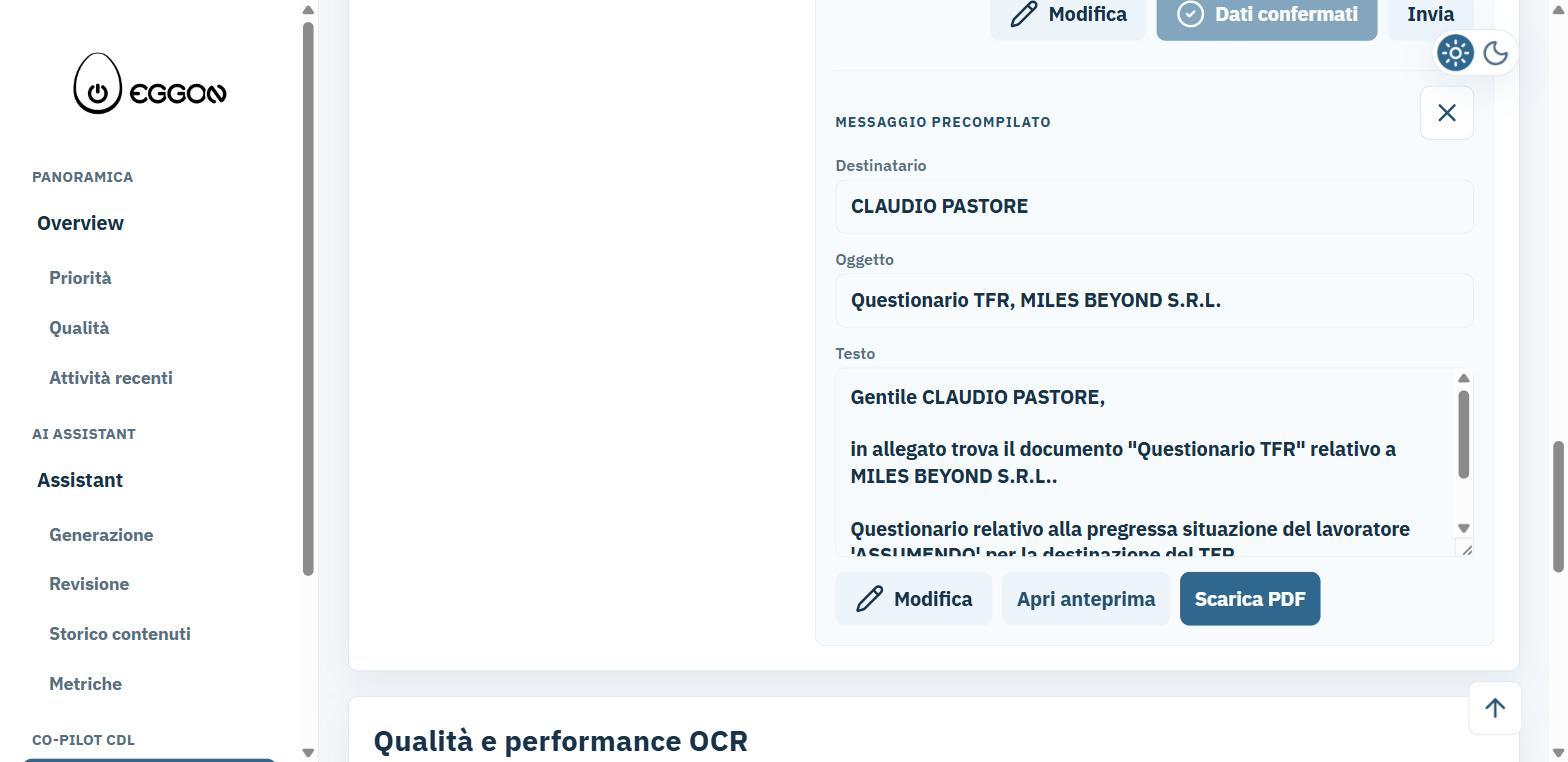
\includegraphics[width=\textwidth]{immagini/copilot-messaggio.png}
\caption{Pannello del messaggio di invio}
\label{fig:copilot-messaggio}
\end{figure}

\subsubsection{Metriche del Co-Pilot}

La sezione \ui{Qualità e performance OCR} riporta i volumi del tenant:

\begin{itemize}
    \item \ui{Documenti analizzati}: file originali caricati;
    \item \ui{Sotto-documenti rilevati};
    \item \ui{Campi con confidenza}: estrazioni al di sopra della soglia;
    \item \ui{Da verificare};
    \item \ui{Documenti pronti};
    \item \ui{In quarantena}.
\end{itemize}

Non esiste una vista analytics con filtri temporali, grafici di accuratezza o tempo medio di analisi: quelle elaborazioni restano fuori perimetro. Le stesse metriche, in forma compatta, compaiono anche in Overview.

\begin{figure}[H]
\centering
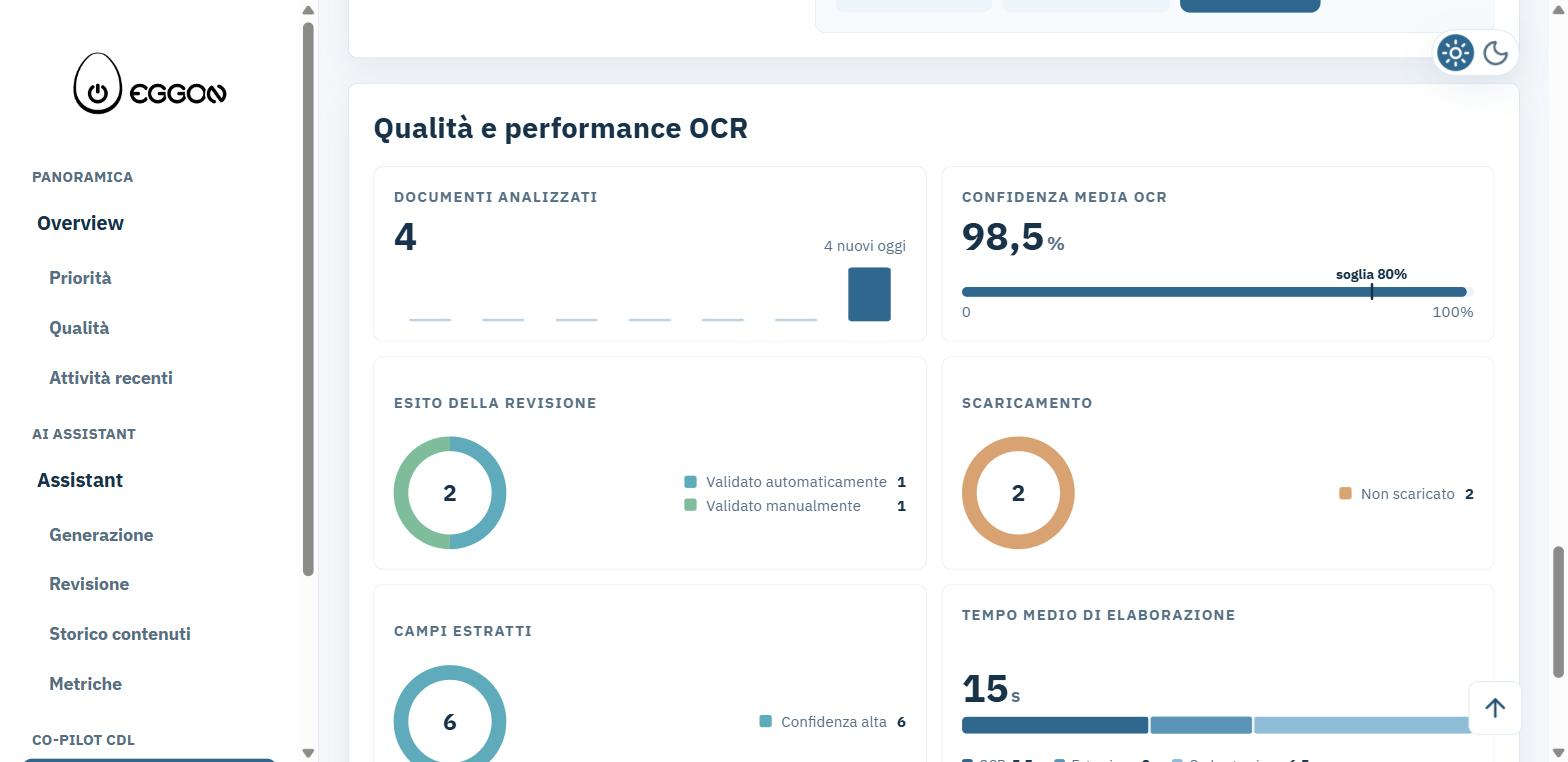
\includegraphics[width=\textwidth]{immagini/copilot-metriche.png}
\caption{Pannello metriche del Co-Pilot}
\label{fig:copilot-metriche}
\end{figure}

\section{Metriche dell'AI Assistant}

Nell'Overview e, in forma equivalente, nello stato caricato dall'Assistant, il redattore vede:

\begin{itemize}
    \item \ui{Contenuti generati}: totale delle generazioni;
    \item \ui{Bozze generate}: comunicazioni ancora in bozza;
    \item \ui{Valutazioni ricevute}: quante generazioni hanno un \glslink{rating}{rating};
    \item \ui{Media stelle}: media aritmetica dei punteggi, oppure un trattino se non ci sono valutazioni.
\end{itemize}

Non sono presenti grafici per tono e stile, né un filtro temporale sulle metriche. Il segnale di qualità percepita è la valutazione 1--5, unica per generazione.

\section{Problemi frequenti}

\begin{center}
\renewcommand{\arraystretch}{1.3}
\begin{tabularx}{\textwidth}{|p{4.6cm}|X|}
\hline
\rowcolor{gray!20}
\textbf{Sintomo} & \textbf{Cosa fare} \\
\hline
Il browser segnala un certificato non attendibile. & È atteso con il certificato self-signed. Procedere comunque al sito, oppure generare un certificato fidato con \texttt{make trusted-local-tls} e riavviare Traefik. \\
\hline
La pagina non si apre su \texttt{localhost:8443}. & Verificare che \texttt{make setup} sia terminato e che \texttt{/health} e \texttt{/ready} rispondano. Consultare \texttt{make logs}. \\
\hline
\ui{Genera bozza} fallisce subito. & Controllare credenziali e region Bedrock nel \texttt{.env}, poi \texttt{make refresh-runtime}. Senza modello di testo non esiste contenuto sostitutivo. \\
\hline
La bozza c'è ma manca la copertina. & Comportamento previsto se il modello immagini non è raggiungibile. Si può caricare un'immagine propria o procedere senza. \\
\hline
Il pulsante di generazione non parte. & Il prompt deve avere almeno 12 caratteri. Completare tono e stile (hanno già un default). \\
\hline
La generazione non compare nello storico. & Premere \ui{Salva nello storico}. Solo lo stato \ui{Approvata} entra nell'elenco. \\
\hline
Il PDF viene rifiutato. & Usare un PDF non cifrato, massimo 20~MB e 50 pagine, con firma \texttt{\%PDF-} valida. Un solo file per volta. \\
\hline
L'analisi resta in coda o fallisce. & Attendere l'aggiornamento in tempo reale. Se lo stato è \ui{Fallito}, aprire il dettaglio e leggere il messaggio: non rilanciare un ``retry'' dall'interfaccia, ricaricare un file corretto. \\
\hline
L'email del destinatario è vuota. & Va compilata a mano in revisione: la pipeline non la estrae. \\
\hline
\ui{Inviato} non corrisponde a una mail partita. & Lo stato cambia allo scaricamento del PDF del messaggio. L'invio reale è fuori dalla MVP. \\
\hline
\end{tabularx}
\end{center}

\section{Appendice: elenco delle schermate da catturare}

Le immagini vanno salvate in \texttt{PB/Manuale Utente/immagini/} con i nomi indicati, a larghezza desktop, tema chiaro, senza dati personali reali. Dopo il salvataggio, sostituire nel sorgente \LaTeX{} ogni \texttt{\textbackslash screenshottodo} con un \texttt{\textbackslash includegraphics} dello stesso file.

\begin{center}
\renewcommand{\arraystretch}{1.25}
{\footnotesize
\begin{longtable}{|p{5.4cm}|p{9.0cm}|}
\hline
\rowcolor{gray!20}
\textbf{File} & \textbf{Inquadratura} \\
\hline
\endfirsthead
\hline
\rowcolor{gray!20}
\textbf{File} & \textbf{Inquadratura} \\
\hline
\endhead
\texttt{shell-completa.png} & Finestra intera sulla Overview, sidebar inclusa. \\
\hline
\texttt{sidebar-navigazione.png} & Solo sidebar, voce attiva visibile. \\
\hline
\texttt{header-tema.png} & Header NEXUM con pulsante tema. \\
\hline
\texttt{overview-hero.png} & Introduzione Overview e pulsanti di avvio. \\
\hline
\texttt{overview-metriche.png} & Priorità, metriche strumenti, attività recenti. \\
\hline
\texttt{assistant-composizione.png} & Form ``Crea una bozza'' compilato. \\
\hline
\texttt{assistant-avanzamento.png} & Barra di generazione in corso. \\
\hline
\texttt{assistant-revisione.png} & Anteprima completa di una bozza con copertina. \\
\hline
\texttt{assistant-modifica.png} & Titolo e testo in modifica. \\
\hline
\texttt{assistant-valutazione.png} & Blocco stelle e commento. \\
\hline
\texttt{assistant-azioni.png} & Pulsanti storico / rigenera / scarta (e conferma scarto). \\
\hline
\texttt{assistant-filtri.png} & Filtri dello storico. \\
\hline
\texttt{assistant-configurazioni.png} & Preset salvati. \\
\hline
\texttt{assistant-storico.png} & Card dello storico, una selezionata. \\
\hline
\texttt{copilot-caricamento.png} & Upload con metadati. \\
\hline
\texttt{copilot-avanzamento.png} & Barra di elaborazione documento. \\
\hline
\texttt{copilot-storico.png} & Tabella storico documenti. \\
\hline
\texttt{copilot-filtri.png} & Filtri documenti. \\
\hline
\texttt{copilot-dettaglio.png} & Anteprima PDF e dati estratti affiancati. \\
\hline
\texttt{copilot-revisione.png} & Campi in modifica, possibilmente con errore di validazione. \\
\hline
\texttt{copilot-messaggio.png} & Messaggio di invio precompilato. \\
\hline
\texttt{copilot-metriche.png} & Card metriche OCR. \\
\hline
\end{longtable}
}
\end{center}

\end{document}
